\setchapterpreamble[u]{\margintoc}
\chapter{Results}
\labch{HESE12}
The 7.5 years of HESE data (2010-2017) was previously used to measure the composition of astrophysical neutrino flavors \sidecite{Juliana_paper} (in particular to search for $\nu_{\tau}$ events) and energy spectrum \sidecite{HESE7_sample}. This dataset included 102 events, (of which 60 events were above 60 TeV), that passed the HESE selection criteria, as outlined in section \ref{sec:HESE}. Two events were identified as Double Cascade candidates using the particle identifier described in section \ref{sec:PID}. 

For this iteration, the analysis has undergone significant changes compared to previous versions while maintaining consistent selection criteria and particle identification methods. The most notable difference lies in the ice model, specifically its properties and influence on the reconstruction of tau decay length, detailed in section \ref{sec:icemodel}. The SPICE-Bfr may have impacts on the overall energy estimates, as the number of photons collected in a given time window have significantly changed in this model of ice depending on the alignment of DOMs with respect to the iceflow axis \sidecite{BFR_paper}. Furthermore, the treatment of detector systematics has evolved, utilizing the SnowStorm method (see section \ref{sec:snowstorm}) instead of discrete Monte Carlo simulation sets used previously. The update also includes revised reconstruction tables \sidecite{updated_recotables_tianlu} for the maximum likelihood reconstruction method described in section \ref{sec:reco}. Additionally, various corrections have been applied to monte carlo simulations, encompassing reweighting to incorporate corrections due to tau polarization and initial state radiation corrections to the Glashow cross-sections (see section \ref{sec:PID}). Lastly, some of the nuisance parameters and analysis software are also different (see section \ref{sec:components}). As a first step, the 7.5 years of HESE data were re-unblinded due to these changes.

This chapter presents flavor measurements made using ~12 years (11.69 to be exact) of HESE data. It begins by discussing the re-unblinding of 7.5 years of data, followed by results from the 12-year fit, including Data-Monte Carlo agreement and detailed post-unblinding checks. Finally, the flavor measurement results are presented and interpreted in the last sectinons.

\section{(Re)Unblinding of 7.5 years of HESE Data}
\label{sec:HESE7}
The re-unblinding of the HESE-7.5 data provided new insights, revealing that 64 events met the HESE selection criteria, each with a deposited energy exceeding 60 TeV. It included 6 Double Cascade events\footnote{Unless explicitly specified, all mentioned classifications are by using SPICEBfr, the default icemodel of the analysis presented in this thesis. At some places in this section, specific comparisons are shown using SPICE-3.2.1}, which is a significant increase from the previous analysis that identified only two Double Cascade events. Notably, 4 of the additional events had initially been classified as single cascades. The reclassification was largely driven by the application of the energy asymmetry cut, which proved to be a crucial factor in differentiating between single and double cascades (see section \ref{sec:PID}). A key difference in this re-unblinding was the icemodel used for reconstruction, as mentioned before. Hence, the data was processed using both SPICE-3.2.1 (used in previous iteration) and SPICE-Bfr to make direct comparisons with the previous results. Using SPICE-3.2.1, reunblinded data contained total of 62 HESE events above 60 TeV deposited energy, of which 7 events were classified as Double Cascades. Moreover, of these 6 and 7 observed Double Cascades, using different ice models, only 3 are common, landing 7 new candidate events. Despite the changes in the total number of classified events, the two common Double Cascade events identified in both iterations exhibited nearly identical reconstructed properties, as outlined in \reftab{reco_values_comparisons_spice} (for SPICE-3.2.1). \todo{should there be a similar table for bfr??} %and \reftab{reco_values_comparisons_bfr} (for SPICEBfr)   


% \begin{table*}[h!]
%     \caption{Comparison of Reconstructed quantities of events classified as Double Cascades upon re-unbling 7.5 years of HESE data  using \textbf{SPICEBfr icemodel} with previous results (grey cells). Shown in the table are (from left), MJD (Modified Julian Date), reconstructed length, reconstructed Energy of first ($\mathrm{E}_1$) and second ($\mathrm{E}_2$) cascades, Energy asymmetry ($\mathrm{E}_\mathrm{A}$), Energy Confinement ($\mathrm{E}_\mathrm{C}$) and classified morphology of the event. The two common events, 57134 (\emph{Double Double}) and 56265 (\emph{Big Bird}) have nearly identical reconstructed quantities.}
%     \labtab{reco_values_comparisons_bfr}
%     \begin{tabular}{c|cc|cc|cc|cc|cc|cc}
%         \toprule
%          MJD    & \multicolumn{2}{c|}{Length}
                
%                         & \multicolumn{2}{c|}{$\mathrm{E}_\mathrm{1}$}
%                                 & \multicolumn{2}{c|}{$\mathrm{E}_\mathrm{2}$} 
%                                     & \multicolumn{2}{c|}{$\mathrm{E}_\mathrm{A}$} 
%                                         & \multicolumn{2}{c|}{$\mathrm{E}_\mathrm{C}$}  
%                                             & \multicolumn{2}{c}{morphology}                \\
                       
%         \midrule
%         57835   &   13 m   & \cellcolor{lightgray}66 m    & 19 TeV   &   \cellcolor{lightgray}79 TeV  &   73 TeV  &   \cellcolor{lightgray}3 TeV  &   -0.58  &   \cellcolor{lightgray}0.93 & 1 &  \cellcolor{lightgray}1&Double& \cellcolor{lightgray}Single\\
%             % \hline
%         57134   &   17 m   & \cellcolor{lightgray}17 m    & 5.7 TeV   &   \cellcolor{lightgray}8.7 TeV  &   92 TeV  &   \cellcolor{lightgray}79 TeV  &   -0.89  &   \cellcolor{lightgray}-0.80 & 0.99 &  \cellcolor{lightgray}0.99&Double& \cellcolor{lightgray}Double\\
%             % \hline
%         56603   & 13 m   & \cellcolor{lightgray}70 m    & 32 TeV   &   \cellcolor{lightgray}85 TeV  &    48 TeV  &   \cellcolor{lightgray}1 TeV  &   -0.19  &   \cellcolor{lightgray}1 & 1 &  \cellcolor{lightgray}0.99 & Double & \cellcolor{lightgray}Single\\
%             % \hline
%         55714   &   14 m   & \cellcolor{lightgray}26 m    & 5 TeV   &   \cellcolor{lightgray}58 TeV  &   82 TeV  &   \cellcolor{lightgray}16 TeV  &   -0.88  &   \cellcolor{lightgray}0.55 & 0.99 &  \cellcolor{lightgray}1&Double& \cellcolor{lightgray}Single\\
%             % \hline
%         55800   &   13 m   & \cellcolor{lightgray}20 m    & 128 TeV   &   \cellcolor{lightgray}133 TeV  &   72 TeV  &   \cellcolor{lightgray}38 TeV  &   0.28  &   \cellcolor{lightgray}0.55 & 1 &  \cellcolor{lightgray}0.99&Double& \cellcolor{lightgray}Single\\
%             % \hline
%         56265   &  16 m   & \cellcolor{lightgray}16 m    & 1.1 PeV   &   \cellcolor{lightgray}1.2 PeV  &   0.9 PeV  &   \cellcolor{lightgray}0.6 PeV  &   0.09  &   \cellcolor{lightgray}0.29 & 1 &  \cellcolor{lightgray}1&Double& \cellcolor{lightgray}Double\\
%             \bottomrule
%     \end{tabular}
% \end{table*}

\begin{table*}[h!]
    \caption{Comparison of Reconstructed quantities of events classified as Double Cascades upon re-unbling 7.5 years of HESE data using \textbf{SPICE-3.2.1 icemodel} with previous results (grey cells). Shown in the table are (from left), MJD (Modified Julian Date), reconstructed length, reconstructed Energy of first ($\mathrm{E}_1$) and second ($\mathrm{E}_2$) cascades, Energy asymmetry ($\mathrm{E}_\mathrm{A}$), Energy Confinement ($\mathrm{E}_\mathrm{C}$) and classified morphology (as per previous anlaysis) of the event. The two common events, 57134 (\emph{Double Double}) and 56265 (\emph{Big Bird}) have nearly identical reconstructed quantities. The most striking differences here are specifically reconstructed length and the fact that $\mathrm{E}_1$ and $\mathrm{E}_2$ seem to be almost flipped for some events, even though reconstructed directions (zenith and azimuth, not shown in the table) remains almost idnetical. The change in $\mathrm{E}_1$ and $\mathrm{E}_2$ changes the $\mathrm{E}_\mathrm{A}$, which is the discrimation cut between single and double cascades.}
    \labtab{reco_values_comparisons_spice}
    \begin{tabular}{c|cc|cc|cc|cc|cc|c}
        \toprule
         MJD    & \multicolumn{2}{c|}{Length}
                
                        & \multicolumn{2}{c|}{$\mathrm{E}_\mathrm{1}$}
                                & \multicolumn{2}{c|}{$\mathrm{E}_\mathrm{2}$} 
                                    & \multicolumn{2}{c|}{$\mathrm{E}_\mathrm{A}$} 
                                        & \multicolumn{2}{c|}{$\mathrm{E}_\mathrm{C}$}  
                                            & \multicolumn{1}{c}{morphology}                \\
                       
        \midrule
        57677   &   27 m   & \cellcolor{lightgray}37 m    & 3.1 TeV   &   \cellcolor{lightgray}128 TeV  &   148 TeV  &   \cellcolor{lightgray}4 TeV  &   -0.96  &   \cellcolor{lightgray}0.94 & 1 &  \cellcolor{lightgray}0.99& \cellcolor{lightgray}Single\\
            % \hline
        57134   &   16 m   & \cellcolor{lightgray}17 m    & 18 TeV   &   \cellcolor{lightgray}8.7 TeV  &   92 TeV  &   \cellcolor{lightgray}79 TeV  &   -0.89  &   \cellcolor{lightgray}-0.80 & 0.99 &  \cellcolor{lightgray}0.99& \cellcolor{lightgray}Double\\
            % \hline
        56763   & 10.2 m   & \cellcolor{lightgray}84 m    & 63 TeV   &   \cellcolor{lightgray}107 TeV  &    87 TeV  &   \cellcolor{lightgray}17 TeV  &   -0.16  &   \cellcolor{lightgray}0.72 & 0.99 &  \cellcolor{lightgray}0.99  & \cellcolor{lightgray}Single\\
            % \hline
        55477   &   14 m   & \cellcolor{lightgray}279 m    & 70 TeV   &   \cellcolor{lightgray}184 TeV  &   84 TeV  &   \cellcolor{lightgray}67 TeV  &   -0.09  &   \cellcolor{lightgray}0.46 & 0.99 &  \cellcolor{lightgray}0.98& \cellcolor{lightgray}Single\\
            % \hline
        55800   &   12 m   & \cellcolor{lightgray}20 m    & 105 TeV   &   \cellcolor{lightgray}133 TeV  &   89 TeV  &   \cellcolor{lightgray}38 TeV  &   0.08  &   \cellcolor{lightgray}0.55 & 1 &  \cellcolor{lightgray}0.99& \cellcolor{lightgray}Single\\
            % \hline

        56221   &  12 m   & \cellcolor{lightgray}12 m    & 209 TeV   &   \cellcolor{lightgray}102 TeV  &   132 TeV  &   \cellcolor{lightgray}237 TeV  &   0.22  &   \cellcolor{lightgray}-0.4 & 0.99 &  \cellcolor{lightgray}0.97& \cellcolor{lightgray}Track\\
            
        56265   &  17 m   & \cellcolor{lightgray}16 m    & 0.8 PeV   &   \cellcolor{lightgray}1.2 PeV  &   1 PeV  &   \cellcolor{lightgray}0.6 PeV  &   -0.08  &   \cellcolor{lightgray}0.29 & 0.99 &  \cellcolor{lightgray}1& \cellcolor{lightgray}Double\\
            \bottomrule
    \end{tabular}
\end{table*}

No matter what icemodel is used, in reunblinding an excess of double cascade events was observed, suggesting the presence of unnoticed changes not already accounted for. Careful search of each step in the particle identification process revealed a significant change in the reconstruction method from the previous iteration. Notably, this change involved the incorporation of high quantum efficiency Digital Optical Modules (DOMs) from DeepCore. In earlier analyses, these DOMs had been excluded from the reconstruction of high-energy neutrino events, in millipede-based reconstructions outlined in \ref{sec:reco}. The rationale for their exclusion stemmed from the smaller statistical uncertainties of digitized waveforms, in compared to the systematic uncertainties. These systematic uncertainties, which were not well-characterized for individual DOMs, could not be factored into the table-based likelihood fitting method. Nonetheless, due to advancements in simulation, including enhanced reconstruction tables and detector simulations, the analysis presented in this thesis included the DeepCore DOMs, hence the next step was to explore why Monte Carlo predictions had underestimated the number of Double Cascade events. 

\begin{figure*}
    \begin{subfigure}[h]{0.7\textwidth}
        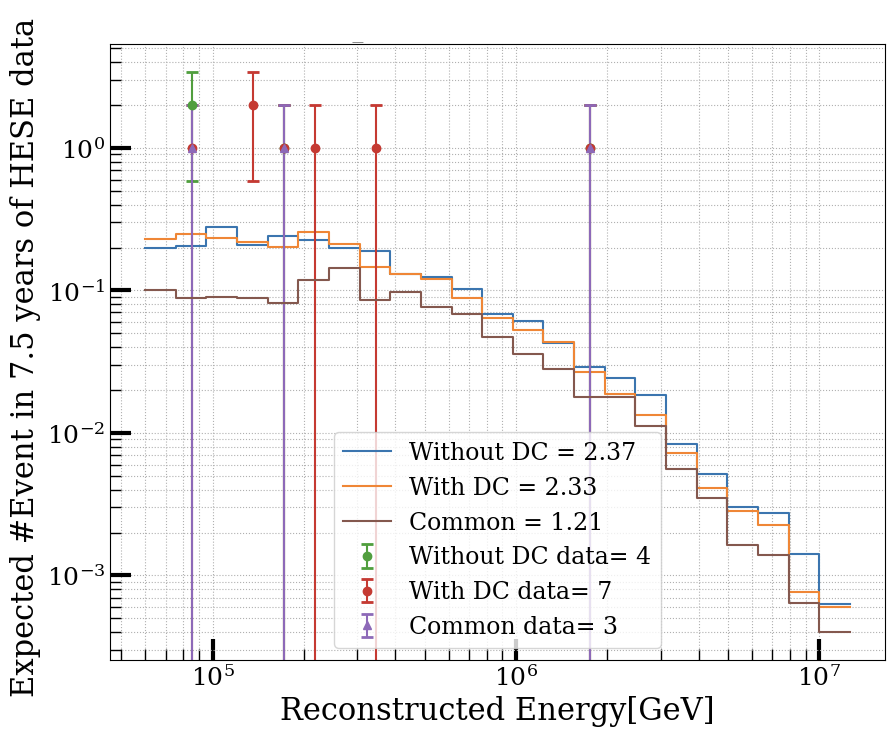
\includegraphics{./figures/results/Spice_DCwithdata.png}
    \end{subfigure}
    \hfill
    \begin{subfigure}[h]{0.7\textwidth}
        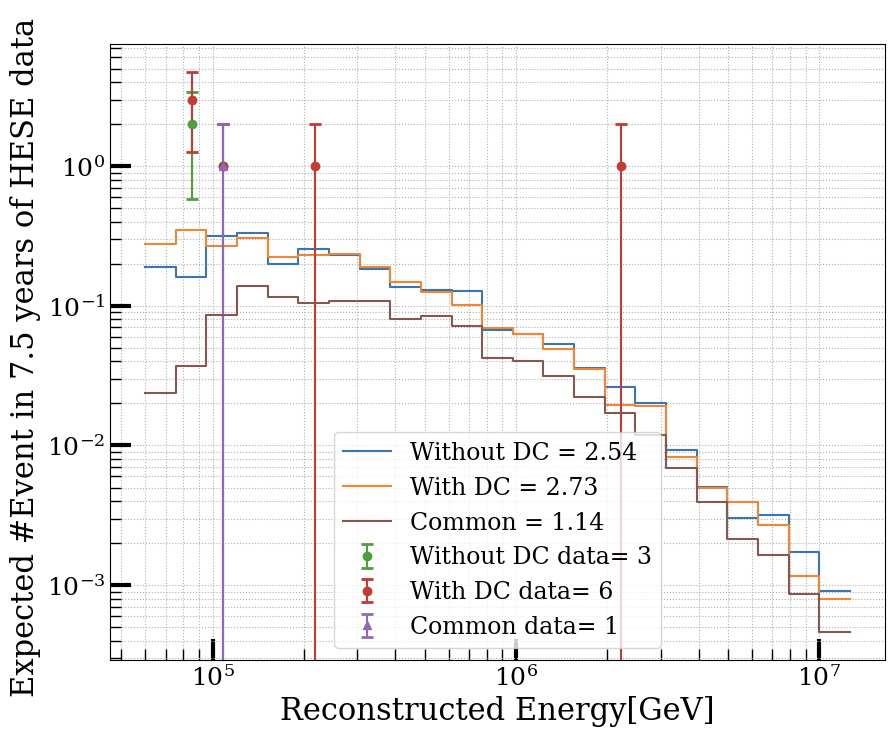
\includegraphics{./figures/results/Bfr_DCwithdata.png}
       
    \end{subfigure}%
    \caption{Distribution of number of expected classified as double cascacdes in 7.5 years of HESE data usign SPICE-3.2.1 (left) and SPICE-Bfr(right) icemodel with (\emph{With DC}) and without (\emph{Without DC}) DeepCore DOMs, along with data events for the respective configurations.}
    \labfig{Bfr_DCwithdata}
\end{figure*}

\reffig{Bfr_DCwithdata} shows the distribution of classified Double Cascade, both with and without the inclusion of DeepCore DOMs. The monte carlo simulations predicts only $\sim 2$ Double Cascade events, yet the data revealed 6 (7) Double Cascade events using SPICE-Bfr (SPICE-3.2.1) when DeepCore DOMs were included and only 3 (4) when they were excluded. It remains clear that no matter what icemodel is used, the distribution of reconstructed energy and overall expectation remains same irrespective of whether DeepCore DOMs are included or not. This discrepancy pointed to potential issues in either the simulation or reconstruction processes involving DeepCore DOMs\todo{In one of the appendix, a short discussion about SPE charge distribution checks done with jvs shall be included}, indicating that further investigation at the monte carlo level is necessary. Such investigations requires efforts that were beyond the timeline of this thesis work and  considering the historical exclusion of DeepCore DOMs (as well as other "bad" DOMs like bright or saturated modules) from reconstruction chains in previous iterations of HESE analyses, this analysis ultimately decided not to include DeepCore DOMs in the full sample unblinding. Ultimately, the re-unblinding of the HESE-7.5 data resulted in 62 events with deposited energies above 60 TeV. Of these, 45 were classified as single cascades, 3 as Double Cascades, and 14 as track events. A detailed comparison between these  reunblinded results and previous results, including classified morphologies (with different iterations of icemodels and DeepCore inclusion/exclusion) is shown in \reftab{HESE7_eventcomparisons}.

\begin{table*}[h]
    \caption[Event classification of 7.5 years of HESE data]{Event classification of 7.5 years of HESE data (Previous) compared with reunblinded sample outcome (all events have Reconstructed total energy > 60 TeV ). The comparison is shown for all 2 different icemodels, each of which further broken down into with and without the deepcore doms. The final outcome of this reunblinding, in order to move forward with the full sample is the last column (without DeepCore using SPICEBfr).}
    \labtab{HESE7_eventcomparisons}
    \raggedright
    \begin{tabular}{ c|c|c c |cc}
        \toprule
            & & \multicolumn{4}{c}{Reunblinded}\\
            
           Morphology&Previous & \multicolumn{2}{c|}{SPICE-3.2.1} & \multicolumn{2}{c}{SPICE-Bfr}\\
           
                     &   & DeepCore & No DeepCore & DeepCore & No DeepCore\\
                                
        \hline
        Cascades & 41 & 41 & 44 &42&45 \\
        Double Cascades & 2 & 7 &4&6& 3 \\
        Tracks& 17&14&14&16&14\\
        \hline
        Total & 60 & 62 &62&64&62\\
        \bottomrule
\end{tabular}
\end{table*}


\section{Unblinding of 12 years of HESE data}
\label{sec:HESE12}
The High-Energy Starting Events (HESE) sample, covering approximately 12 years of IceCube detector live time (4268.7 days) from 2010 to August 2022, was unblinded in January 2024 for the analysis outlined in Section 4.3. This sample includes 167 events that passed the HESE selection criteria, which involved the veto and total charge conditions as detailed in Section 4.2. Of these, 3 were coincident events that had previously been removed by manual inspection, but were retained this time since the current Monte Carlo simulations now account for such coincidences. Despite this, the energy threshold of 60 TeV effectively filtered them out, resulting in a final sample of 97 events above the 60 TeV deposited energy threshold. Using the ternary topology identification method from this thesis, 64 events were classified as single cascades, 5 as double cascades, and 28 as tracks.



\subsection{Fit results}
\label{sec:HESE12_fitresults}

\subsubsection{Blind Fit results}
\label{blindfit}
In IceCube, all the analysis are done in a blind fashion, meaning reconstruction and other fit details are applied to simulation to produce expectations in form of Monte Carlo PDFs and later data is fit to this expectation to make the desired measurement. Details of such a fit are given in \ref{sec:analysis}. For such fits, before looking at the full data results, sometimes a middle step is considered where only nuisance parameters are revealed first (and/or only background region is looked at) to see any striking disagreement between the data and monte carlo or unexplainable behaviour of any nuisance parameters (e.g. if they are hitting the fit range boundary etc).  Stopping criterions are set-up beforehand in case this step shows any troublesome results. For HESE sample, since overall expectation is quite low, looking at a subsample would certainly be unyielding. Thus, blindfit for this analysis included observing the nuisance parameters behaviour and goodness of the fit. The stopping criterions included, minimum p-value of 5\% for the goodness of fit test (see \ref{sec:analysis} for details) and applying priors on systematics in case they hit the boundary. These priors are derived from the so far gathered best knowledge of the ice and detector, and were tested by running pseudo trials (see \ref{sec:hists}) to test their effects on signal distributions. As a post-unblinding check, they are to be removed to see if any significant changes are observed in signal parameters. 

The bestfir values of nuisance parameters are summarized in \reftab{bf_nuisance} along with their gaussian priors. Initially, the holeice parameters, $\eta_{\mathrm{h.ice-p0}}$ and $\eta_{\mathrm{h.ice-p1}}$ were hitting the boundary, but upon applying the tested priors this effect was resolved. As a post unblinding check, these priors were removed to check any changes in signal parameters, no such significant changes were observed. The likelihood includes a penalty term (see \ref{sec:analysis}) which was checked for the 2D scan of flavour ratio triangle to see the effect of pulls due to this prior. \todo{perhaps the triangle plot showing llh penalty due to these priors can be shown here? or should this discussion have its separate appendix?}    

\begin{figure}[ht]
	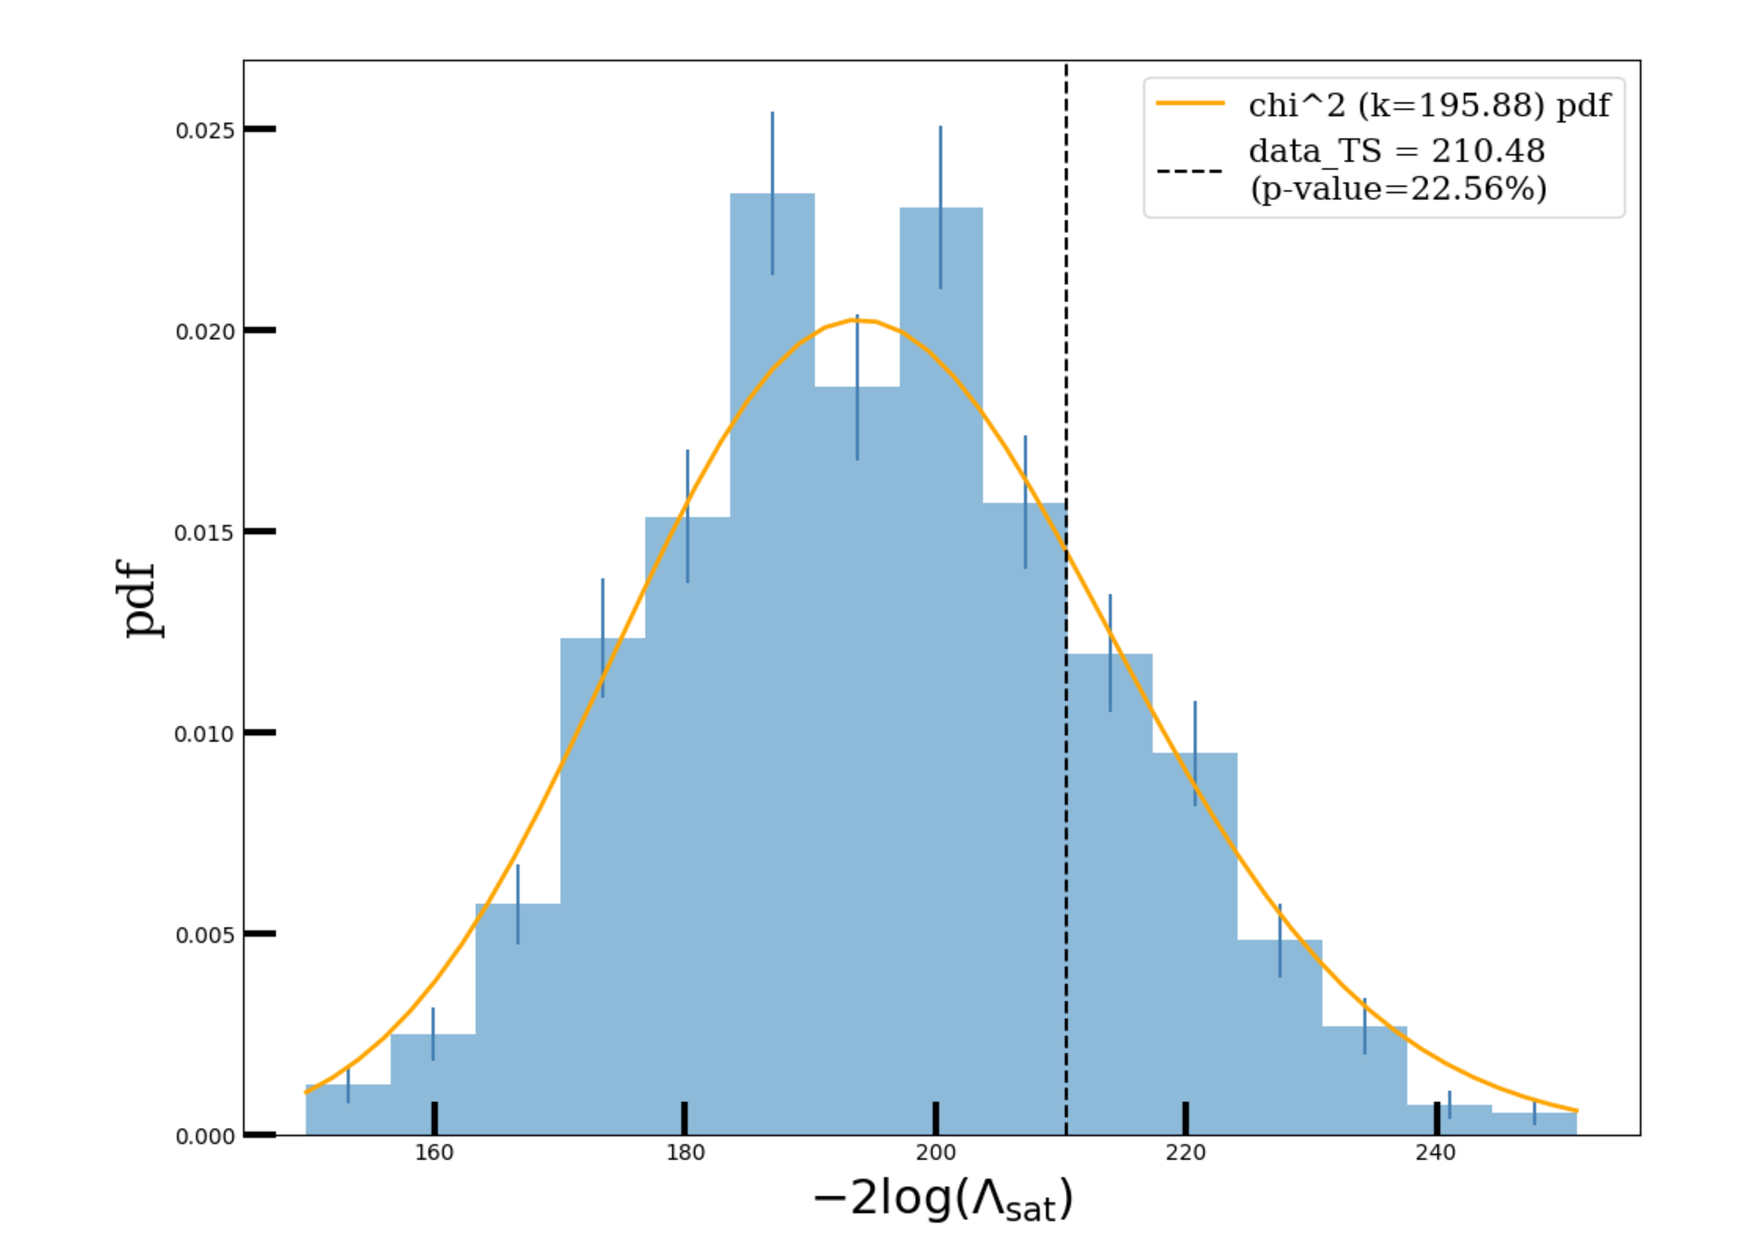
\includegraphics[scale=0.5]{./figures/results/GOF.pdf}
	\caption{Distribution of the test statistics for 1000 pseudotrials injected at bestfit (signal parameters kept blind). Veritcal line shows TS of data, which matches quite well with degrees of freedom derived by fitting a $\chi^2$ to the distribution.}
    \labfig{gof}
\end{figure}

Most of the nuisance parameters are primarily fitted to their priors with minimal deviations from the modeled uncertainties. The detector systematics are set away from default values, although they still remain within one standard deviation of the applied prior width. This can be explained as follows: The method used to apply systematic uncertainties, known as the "gradient method" (see \ref{sec:params}), in the fit assumes linearity whether moving away from or towards the central value. In an ideal scenario, the range within which the parameter is allowed to vary (and the simulation range) should be narrow enough that the central value can always be recovered. However, these parameters are considered only as nuisance in the fit, and they are not meant to be measured. Furthermore, the detector is not so precisely calibrated as to know the true value of these parameters. Therefore, in practice, the range is kept quite wide. In the analysis presented here, where the overall expectation is low and the data is binned in histograms, such things can happen, causing the nuisance parameters to shift.  In order to save computational power, the gradients are calculated once for a given spectrum assumption. If the underlying spectrum of data is far from this assumed spectrum, small changes in these signal parameters can cause larger deviations. Most of these systematics thus ended up having a gaussian prior in the fit, as listed in the \reftab{bf_nuisance}. 
 
\begin{table*}[h]
    \caption{The best-fit parameter values of the nuisance parameters. The uncertainties are calculated at the 68\% confidence level through a profile likelihood scan assuming Wilks' theorem, in case of a flat likelihood space, fit boundaries are given as limits. Last column states the gaussian priors on the parameters (if applicable) in terms of the mean ($\mu$) and width ($\sigma$). The table is divided in terms of type of the nuisance parameters, above part includes all the parameters that affects the atmosphgeric neutrino components and the lower part consists if parameters stemming through various detector components. For details, see \ref{sec:params}}
    \labtab{bf_nuisance}
    {\renewcommand{\arraystretch}{1.4}
    \begin{tabular}{ c c |c|c}
        \hline
        \multicolumn{2}{c|}{Parameter}  & Best-Fit value & Prior ($\mu,\sigma$)\\
        \hline
        \hline
        $\Phi_{\mathrm{conv}}$& Conventional Flux normalisation & $0.99_{-0.2}^{+0.19}$ & (1.0,0.2)\\
        \hline
        $\Phi_{\mathrm{prompt}}$& Prompt Flux Normalisation & ${0.0}_{-0.0}^{+2.25}$ & - \\
        \hline
        $\xi_{\mathrm{CR}}$& Interpolation etween Cosmic Ray Models & $0.042_{-1}^{+2}$ & (0,1)\\
        \hline
        $\Delta\gamma_{\mathrm{CR}}$& Cosmic Ray Spectral Index Shift & $-0.00_{-1}^{+1}$ & (0,0.05)\\
        \hline
        $H_{\mathrm{Barr}}$& Barr-parameter modifying the pion-contribution & $0.0_{-0.5}^{+0.5}$ & (0,0.15)\\
        \hline
        $W_{\mathrm{Barr}}$& Barr-parameter modifying the kaon-contribution & $0.0_{-0.5}^{+0.5}$ & (0,0.40)\\
        \hline
        $Y_{\mathrm{Barr}}$& Barr-parameter modifying the pion-contribution & $0.0_{-0.5}^{+0.5}$ & (0,0.30)\\
        \hline
        $Z_{\mathrm{Barr}}$& Barr-parameter modifying the pion-contribution & $0.0_{-0.5}^{+0.5}$ & (0,0.12)\\
        \hline
        $\Phi_{\mathrm{muongun}}$ & Muon Flux Normalisation & $1.16_{-0.43}^{+0.42}$ & (1,0.5)\\
        \hline
        $\mathrm{I}_{\mathrm{scale}}$ & scale factor for Neutrino Nucleon Inelasticity weight & $0.99_{-0.09}^{+0.1}$ & (1,0.1)\\
        \hline
        
        \multicolumn{4}{c}{\textbf{Detector Systematics}}\\
        \hline
        $\eta_{\mathrm{domeff}}$& Optical Efficiency of DOMs & $1.04_{-0.04}^{+0.06}$ & (1.0,0.1)\\
        \hline
        $\eta_{\mathrm{abs}}$& Ice Absorption Scaling & $0.99_{-0.04}^{+0.04}$ & (1.0,0.05)\\
        \hline
        $\eta_{\mathrm{scat}}$& Ice Scattering Scaling & $0.98_{-0.04}^{+0.04}$ & (1.0,0.05)\\
        \hline
        $\eta_{\mathrm{h.ice-p0}}$& parametrization for refrozen icecolumn & $-0.27_{-0.38}^{+0.28}$ & (-0.27,0.5)\\
        \hline
        $\eta_{\mathrm{h.ice-p1}}$& parametrization for refrozen icecolumn & $-0.08_{-0.05}^{+0.04}$ & (-0.042,0.05)\\
        \hline
        $\eta_{\mathrm{aniso}}$& Ice Anisotropy Scaling & $0.99_{-0.63}^{+0.54}$ & -\\
        \hline
        \hline
    \end{tabular}
    }
\end{table*}



Lastly, the goodness of the fit (GOF) is tested by using the pseudo data. This data is genereated by injecting the Best Fit Parameter (BFP) values as the true parameters and then fluctuating the expected bin counts to consider MC uncertainty and Poisson fluctuations in the data. A distribution of Test Statistic (TS) values is then observed, which is derived from the ratio of the fitted likelihood to the saturated Poisson likelihood. The saturated likelihood represents the alternative hypothesis, where the data perfectly matches the assumed model. The saturated Poisson likelihood assumes the most ideal scenario, where each analysis bin observes statistically significant data, following a chi-squared distribution with degrees of freedom equal to the difference between the number of analysis bins and the number of free parameters in the fit. However, in reality, not all bins observe data, so some deviations are expected. By comparing the distribution of TS values from these pseudo-data trials to the distribution derived from the real data, a p-value can be calculated. The p-value represents the probability of finding a TS value from the trials that is at least as large as the one from the data fit. \reffig{gof} illustrates this distribution, where the data TS is compared with the distribution of trial TS values. The obtained p-value is 22.56\%. Based on this test, it is concluded that the fit result is consistent with the expected outcome from the pseudo-data trials.


\subsubsection{Full fit results}
\label{final_fit}
The bestfit values of the signal parameters for the 97 HESE events are summarized in \reftab{bf_signal}. As explained in \ref{sec:params}, the flavour fractions within \texttt{NNMFit} framework are fitted as scaling factors $s_{\nu_{e}}$ and $s_{\nu_{\tau}}$, which modifies the flux of electron and tau neutrinos relative to the muon neutrino flux. Which is why, the signal parameters listed in \reftab{bf_signal} needs to be converted to their corresponding flavour fractions (\todo{reference fraction conversion formula here}), giving us measured flavoured composition of astrophysical neutrinos as, \textbf{$\nu_e:\nu_{\mu}:\nu_{\tau} = 0.19:0.43:0.38$}. Since the measurement is done for the entire spectrum, this value that of best-fit flavour composition which is expected on earth in case neutrinos at high energy sources are produced with muon damped scenario, hints that diffuse neutrino spectrum at high energies (sensitivity range of this analysis is ~ 100TeV-10PeV) may be dominated by sources with such production mechanisms. Nevertheless, the limits derived (see \ref{sec:flavour_results}) cannot reject either of these scenarios with reasonable significance. 

\begin{table*}[h]
    \caption{The best-fit parameter values for the signal parameters for a single power-law model at 100 TeV muon neutrino energy for both particle and antiparticle. The uncertainties are calculated at the 68\% confidence level through a profile likelihood scan assuming Wilks' theorem.}
    \labtab{bf_signal}
    {\renewcommand{\arraystretch}{1.4}
    \begin{tabular}{ c c |c}
        
        \hline
        \multicolumn{2}{c|}{Parameter}  & Best-Fit value\\
        \hline
        \hline
        $\phi_{\nu_{\mu}}$ &astro. $\nu_{\mu}$ normalisation [$10^{-18} \mathrm{GeV}^{-1}\mathrm{cm}^{-2}\mathrm{sr}^{-1}\mathrm{s}^{-1}$]& $2.53_{-1.49}^{+1.78}$\\
        \hline
        $\gamma_{\mathrm{astro}}$ &astro. spectral index & $2.84_{-0.18}^{+0.19}$\\
        \hline
        $s_{\nu_e}$ &astro. $\nu_{e}$ scaling factor to modify total flux norm ($\Phi_{\nu+\bar\nu}^{\mathrm{astro}}$) relative to $\phi_{\nu_{\mu}}$ & $0.45_{-0.40}^{+0.68}$\\
        \hline
        $s_{\nu_{\tau}}$ &astro. $\nu_{\tau}$ scaling factor to modify total flux norm ($\Phi_{\nu+\bar\nu}^{\mathrm{astro}}$) relative to $\phi_{\nu_{\mu}}$ & $0.896_{-0.89}^{+1.34}$\\
        \hline
        \hline
    \end{tabular}
    }
\end{table*}


The best-fit value of astrophysical index ($\gamma_{\mathrm{astro}}$), assuming a single power law is $2.84_{-0.18}^{+0.19}$. This value is in well agreement with the previous results \sidecite{HESE7_sample}. As for the normalization, as per the formulation of the flavour fit within the \texttt{NNMFit} the best-fit value shown in the table is astrophysical $\nu_{\mu}$ normalization, which when converted using appropriate transformations gives the total flux normalization (for all flavours) $\Phi_{\nu+\bar\nu}^{\mathrm{astro}} = 5.94_{-4.28}^{+5.64}$\todo{check this number again!!}. The larger uncertainity on normalization is expected for such a fit where each flavour components are allowed to be free, that in turn have larger uncertainty on them (see \reftab{bf_signal}). 

Lastly, the table in \reftab{pid_comparisons} provides the breakdown of expected events classified into specific morphologies and their individual components. Additionally, the comparison includes the expectation based on a $\nu_e:\nu_{\mu}:\nu_{\tau} = 1:1:1$ flavor ratio, which was determined by running the fit with fixed flavor ratios. It is important to note that the expectation aligns more closely with the data when the flavor ratios are independently fitted.

\begin{table*}[h]
    \caption{The expected number of HESE events, classified into three morphologies, assuming a fixed flavour ratio of 1:1:1 and at the best-fit flavour ratio. The total expected event counts are further broken down into each of the flux components, Astrophysical (Astro), Conventional (Conv), Atmospheric Muons (Muon). Prompt component is not shown here as best-fit value of the prompt norm ($\Phi_{\mathrm{prompt}}$) is 0.}
    \labtab{pid_comparisons}
    
    \begin{tabular}{ c| c c c c |c c c c|c}
        
        \hline
        \makecell{Reconstructed \\ Morphology} & \multicolumn{4}{c|}{$\nu_e:\nu_{\mu}:\nu_{\tau} = 1:1:1$(fixed)}  & \multicolumn{4}{c|}{$\nu_e:\nu_{\mu}:\nu_{\tau} = 0.19:0.43:0.38$ (free)} & Data\\
         &Astro&Conv&Muon&Total&Astro&Conv&Muon&Total& \\
        \hline
        \hline
        Cascades&$58\pm2$&$6.8\pm0.9$&-&\textbf{$65\pm2.7$}&$57\pm2$&$6\pm0.79$&-&\textbf{$63.4\pm2.4$}&\textbf{64}\\
        Tracks&$11.8\pm0.7$&$6.3\pm1$&$2\pm3$&\textbf{$20\pm3.6$}&$16\pm0.8$&$5.7\pm0.9$&$1.84\pm2.7$&\textbf{$23.4\pm3.4$}&\textbf{28}\\
        \makecell{Double \\ Cascades}&$3.2\pm0.3$&$0.4\pm0.2$&-&\textbf{$3.5\pm0.5$}&$3.8\pm0.3$&$0.3\pm0.2$&-&\textbf{$4.1\pm0.4$}&\textbf{5}\\
        \hline
        \hline
    \end{tabular}
    
\end{table*}

\subsection{Data/Monte Carlo Agreement}
\label{sec:data_mc}
Even with a reasonably good fit, any significant mismodeling can only be discerned through a comparison with the Monte Carlo expectations. Nonetheless, the subsequent figures demonstrate the distributions of the analysis observables for all three morphologies, for HESE events with deposited energies above 60 TeV. These plots are generated using the best-fit values described in \reftab{bf_signal} and \reftab{bf_nuisance}. Each figure displays individual components as well as the sum of all components under the label \textbf{MC sum}. Additionally, to highlight any noteworthy features, a ratio plot is included for each distribution, illustrating the ratio of data events to each bin of the MC sum. Although there are observed slight fluctuations, the presence of considerable statistical uncertainties makes it challenging to pinpoint any specific spectral features. 

\reffig{Cascades_datamc} and \reffig{Tracks_datamc} shows the distribution of reconstructed energy (left) and cosine of reconstructed zenith (right) for events classified as single cascades and tracks resepctively in the 12 years of HESE data. The zenith plot clearly illustrates the all-sky selection feature of the HESE sample by overall being flat throughout the zenith distribution. It also highlights the decrease of the conventional component in the downgoing region (cos(zenith>0.25)), indicating the self-veto effect. Additionally, the muongun component is exclusively visible in the track histogram due to fact that the ternary classifier predominantly classifies muons as tracks. However, it's important to note that the expectation exhibits substantial statistical uncertainties due to the lack of sufficient \texttt{muongun} monte carlo. To mitigate the impact of the noisy distribution caused by extensive Monte Carlo uncertainties, a kernel density estimation (KDE) is employed to smoothen out the fluctuations present. While both morphology distributions reveal some minor structures, they do not demonstrate any statistically significant characteristics.

\begin{figure*}[h]
    \begin{subfigure}[h]{0.7\textwidth}
        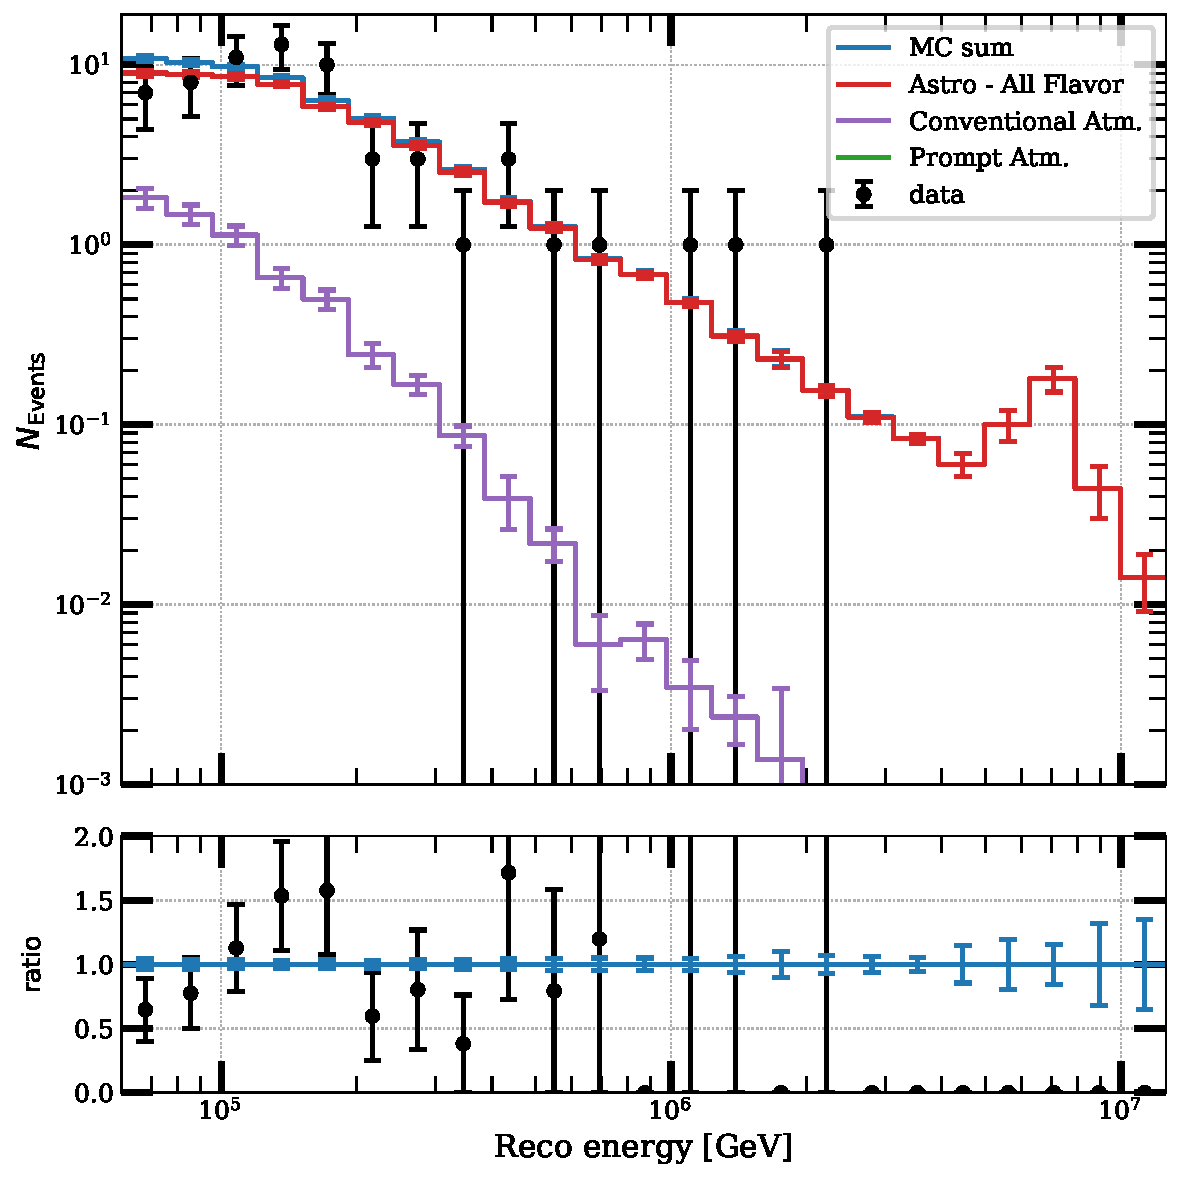
\includegraphics{./figures/results/DataMC_IC86_pass2_SnowStorm_v2_Bfr_Cascades_energy.pdf}
    \end{subfigure}
    \hfill
    \begin{subfigure}[h]{0.7\textwidth}
        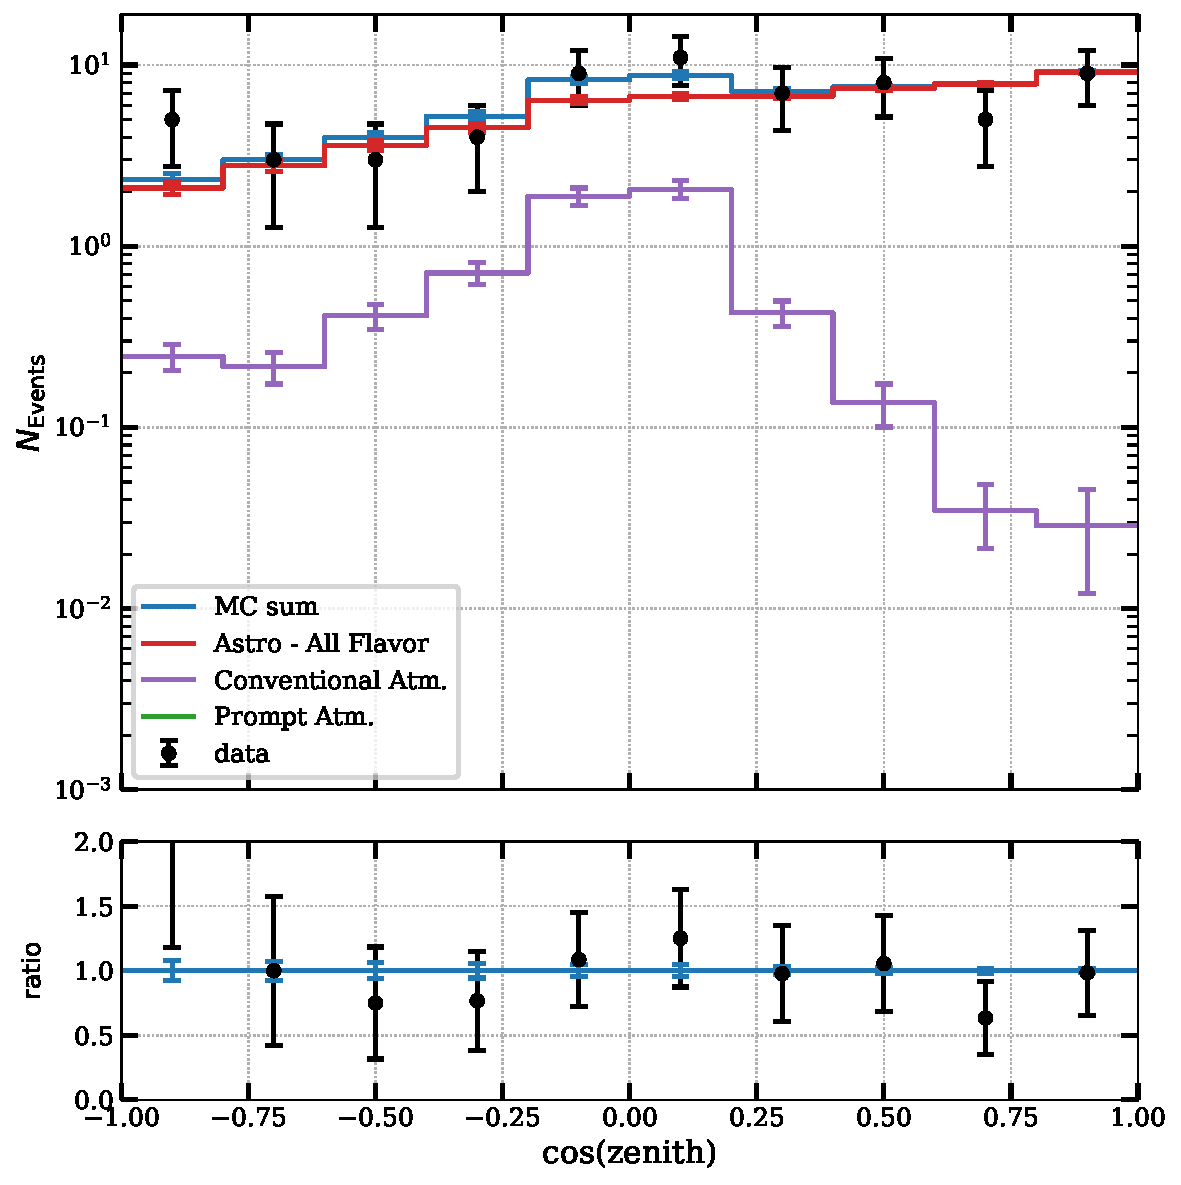
\includegraphics{./figures/results/DataMC_IC86_pass2_SnowStorm_v2_Bfr_Cascades_zenith.pdf}
       
    \end{subfigure}%
    \caption{Observable distributions of the total deposited energy (left) and the zenith angle (right) for events classified as \textbf{single cascades} along with data point positions. Individual components of the fits are produced using bestfit values given in \reftab{bf_signal} and \reftab{bf_nuisance} and MC sum is sum of all of these components. Prompt component is missing on account of bestfit value of 0 for the $\Phi_{\mathrm{prompt}}$.}
    \labfig{Cascades_datamc}
\end{figure*}

\begin{figure*}[h!]
    \begin{subfigure}[h]{0.7\textwidth}
        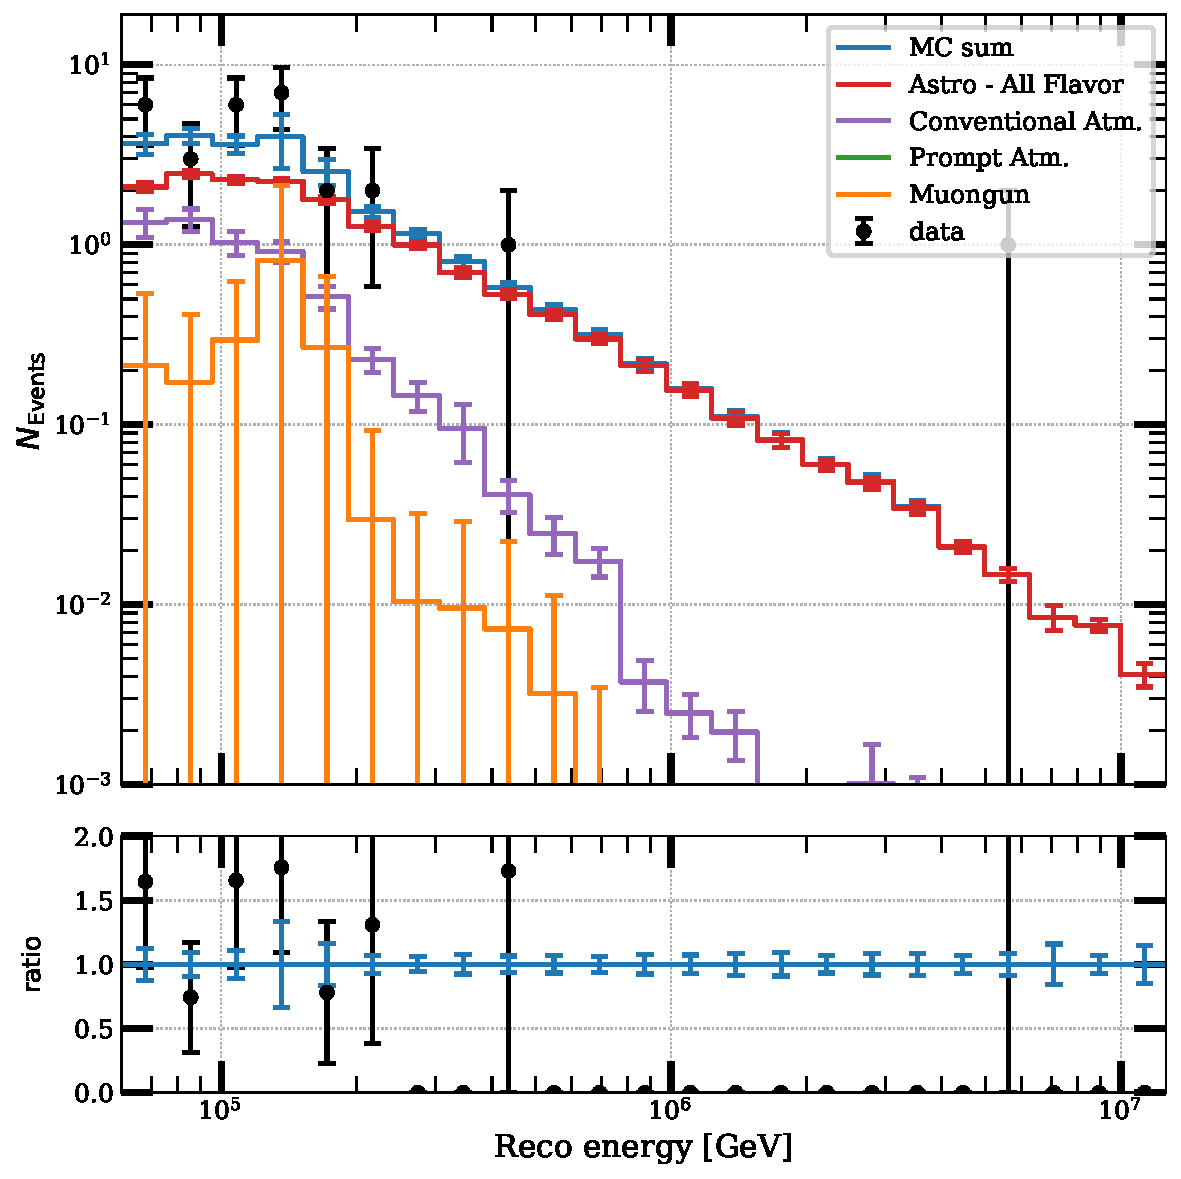
\includegraphics{./figures/results/DataMC_IC86_pass2_SnowStorm_v2_Bfr_Tracks_energy.pdf}
    \end{subfigure}
    \hfill
    \begin{subfigure}[h]{0.7\textwidth}
        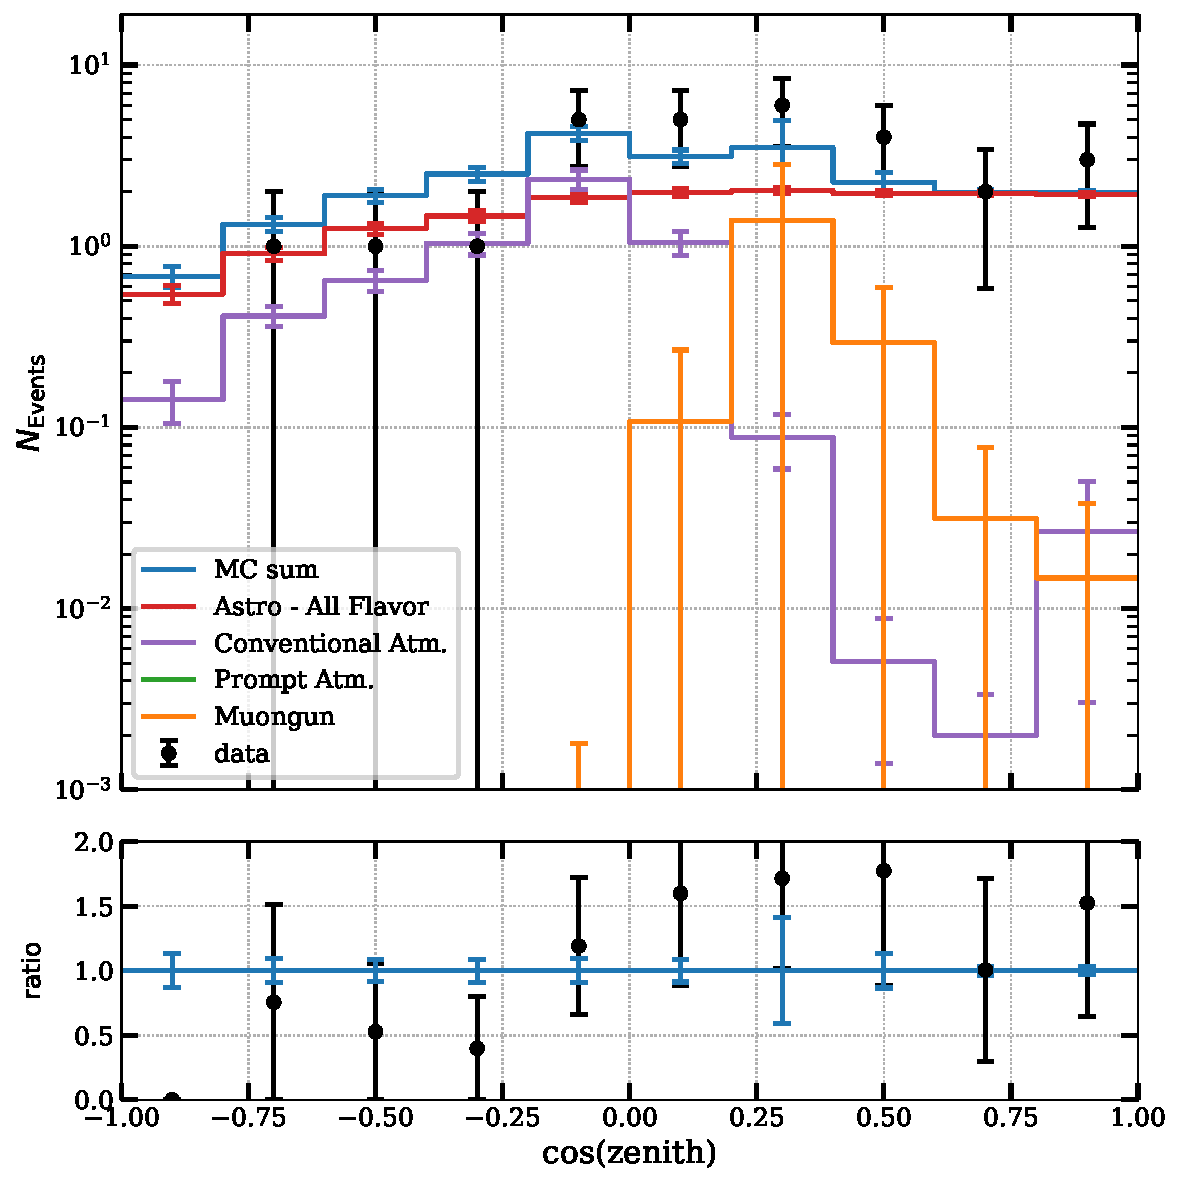
\includegraphics{./figures/results/DataMC_IC86_pass2_SnowStorm_v2_Bfr_Tracks_zenith.pdf}
       
    \end{subfigure}%
    \caption{Observable distributions of the total deposited energy (left) and the zenith angle (right) for events classified as \textbf{tracks} along with data point positions. Individual components of the fits are produced using bestfit values given in \reftab{bf_signal} and \reftab{bf_nuisance} and MC sum is sum of all of these components. Prompt component is missing on account of bestfit value of 0 for the $\Phi_{\mathrm{prompt}}$.}
    \labfig{Tracks_datamc}
\end{figure*}
\newpage
\reffig{double_datamc} illustrates the distribution of reconstructed energy (left) and reconstructed length (right) for events classified as double cascades in the 12 years of HESE data. In the second energy bin, there is an overfluctuation, but it's challenging to incorporate this as a feature due to the large uncertainties in both the monte carlo and data. An interesting feature of the fit can be seen in the conventional component distribution. The application of gradient correction as an additive factor per component indicates that systematics are trying to adjust this component to account for the excess of double cascades at low energy and high length. This suggests that due to fewer statistics compared to tracks, there is more variability in this parameter across the double cascade bins.  Another noteworthy observation is that one event, although close to 100 TeV, has a large length, suggesting that it is a misclassified track. This particular event demonstrates Energy Confinement near the edge (0.97), a cut that is supposed to differentiate between a double cascade and a track, but not quite above the threshold to be a track (0.99). And hence, the event passed all the cuts and ended up being classified as a double cascade. This becomes more evident in 2D distribution of energy and length in \reffig{LvsE_datamc}, where this event clearly ends up in a  background dominated region of the PDF (see \ref{sec:PID} for signal and background pdfs of double cascades). 


\begin{figure*}[h]
    \begin{subfigure}[h]{0.7\textwidth}
        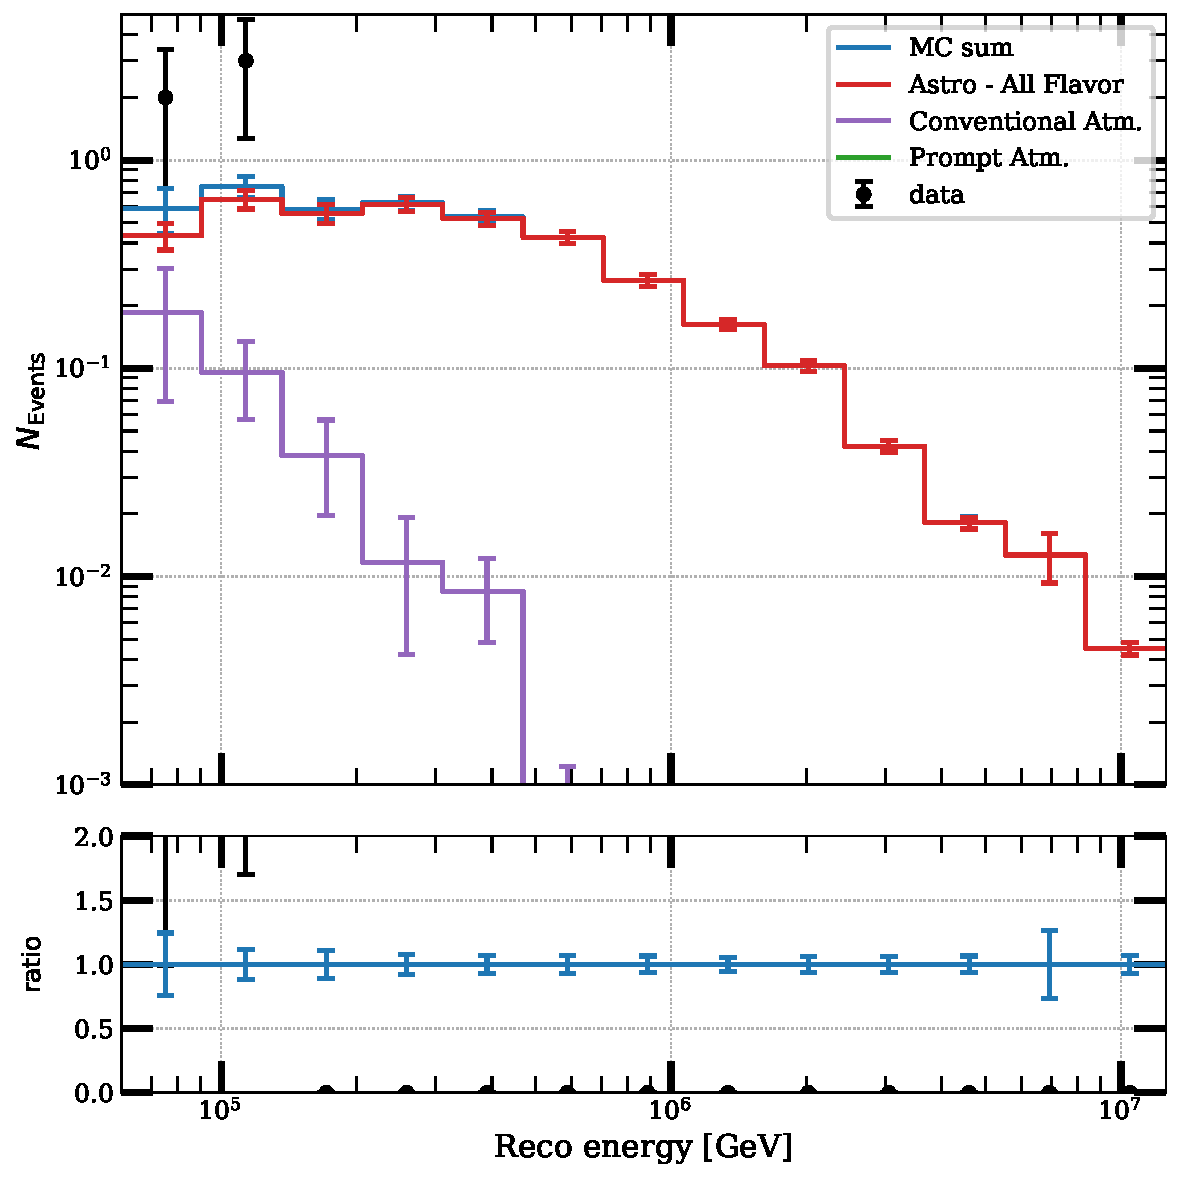
\includegraphics{./figures/results/DataMC_IC86_pass2_SnowStorm_v2_Bfr_DoubleCascades_energy.pdf}
    \end{subfigure}
    \hfill
    \begin{subfigure}[h]{0.7\textwidth}
        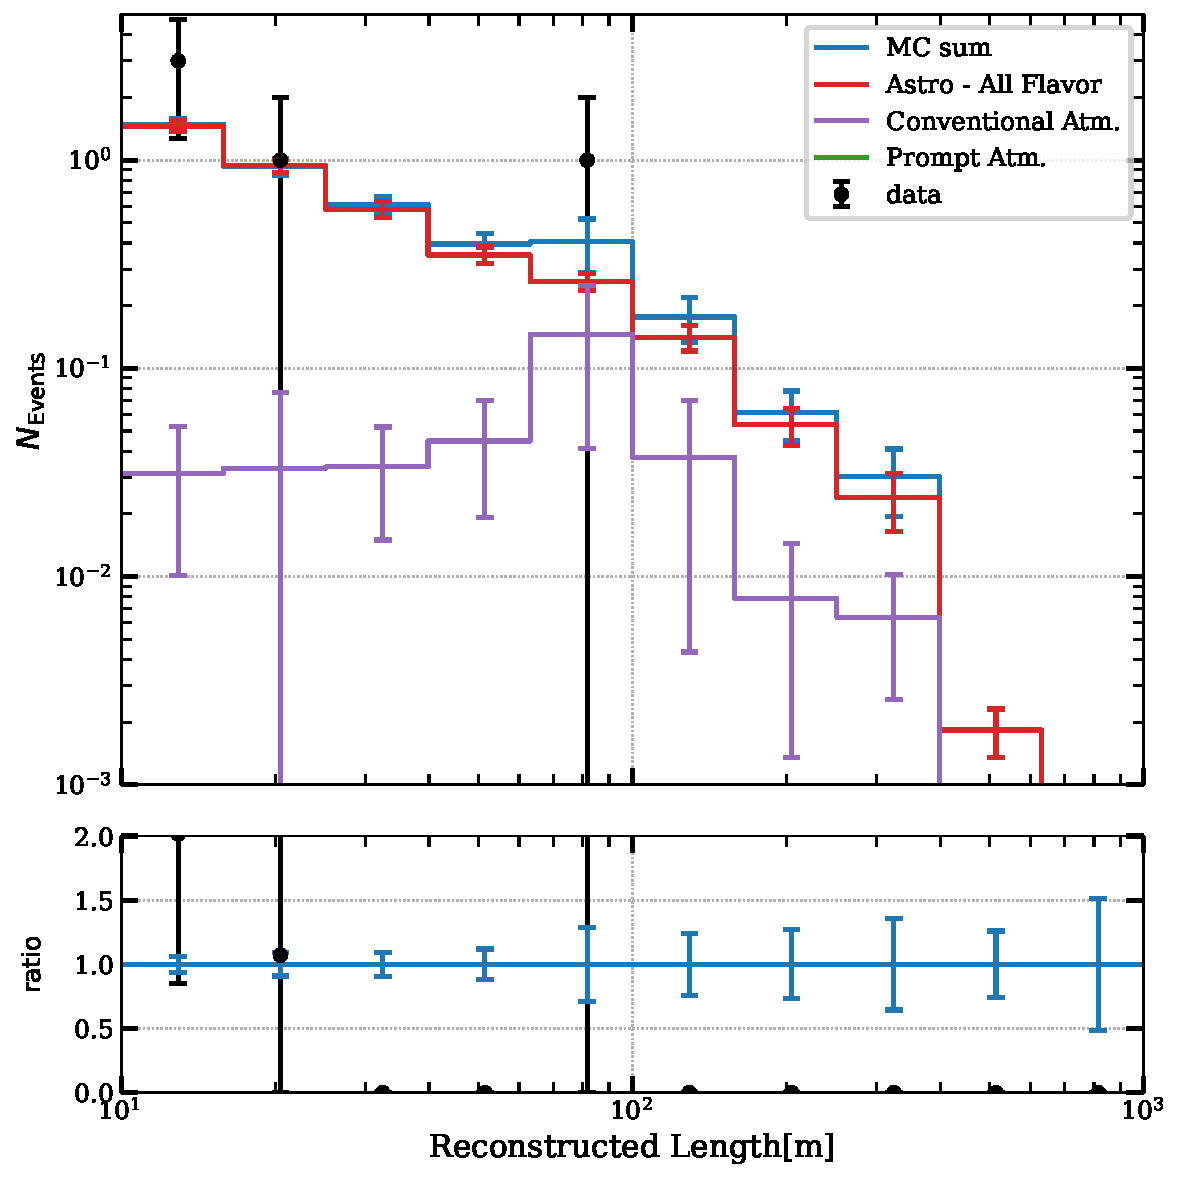
\includegraphics{./figures/results/DataMC_IC86_pass2_SnowStorm_v2_Bfr_DoubleCascades_zenith.pdf}
       
    \end{subfigure}%
    \caption{Observable distributions of the total deposited energy (left) and the reconstructed length (right) for events classified as \textbf{double cascades} along with data point positions. Individual components of the fits are produced using bestfit values given in \reftab{bf_signal} and \reftab{bf_nuisance} and MC sum is sum of all of these components. Prompt component is missing on account of bestfit value of 0 for the $\Phi_{\mathrm{prompt}}$.}
    \labfig{double_datamc}
\end{figure*}
The figure \reffig{LvsE_datamc} illustrates a two-dimensional PID pdf of reconstructed double cascade events, based on the best-fit values described in the tables. The vertical lines demonstrate how quickly the single-cascade background decreases with length. For instance, 68\% of misclassified single cascades have reconstructed double-cascade lengths of less than $\sim 14$ m, 90\% have lengths below $\sim  20$ m, and only 1\% have lengths exceeding $\sim 25$ m. Two of the data events are outside the 68\% region, but one of these events is still within the signal region indicated by white lines. The event with a reconstructed length of approximately 95 m but less than 80 TeV energy is clearly in the background region. Another important observation from this figure is the lack of smoothness expected from PDFs when performing forward folding fits. The gradients are applied as an additive correction per bin, to allow detector systematic variations in the fit. This in turn can significantly change the per bin expectations, making the distributions more fluctuating.
\begin{figure*}[h]
    \begin{subfigure}{0.8\textwidth}
        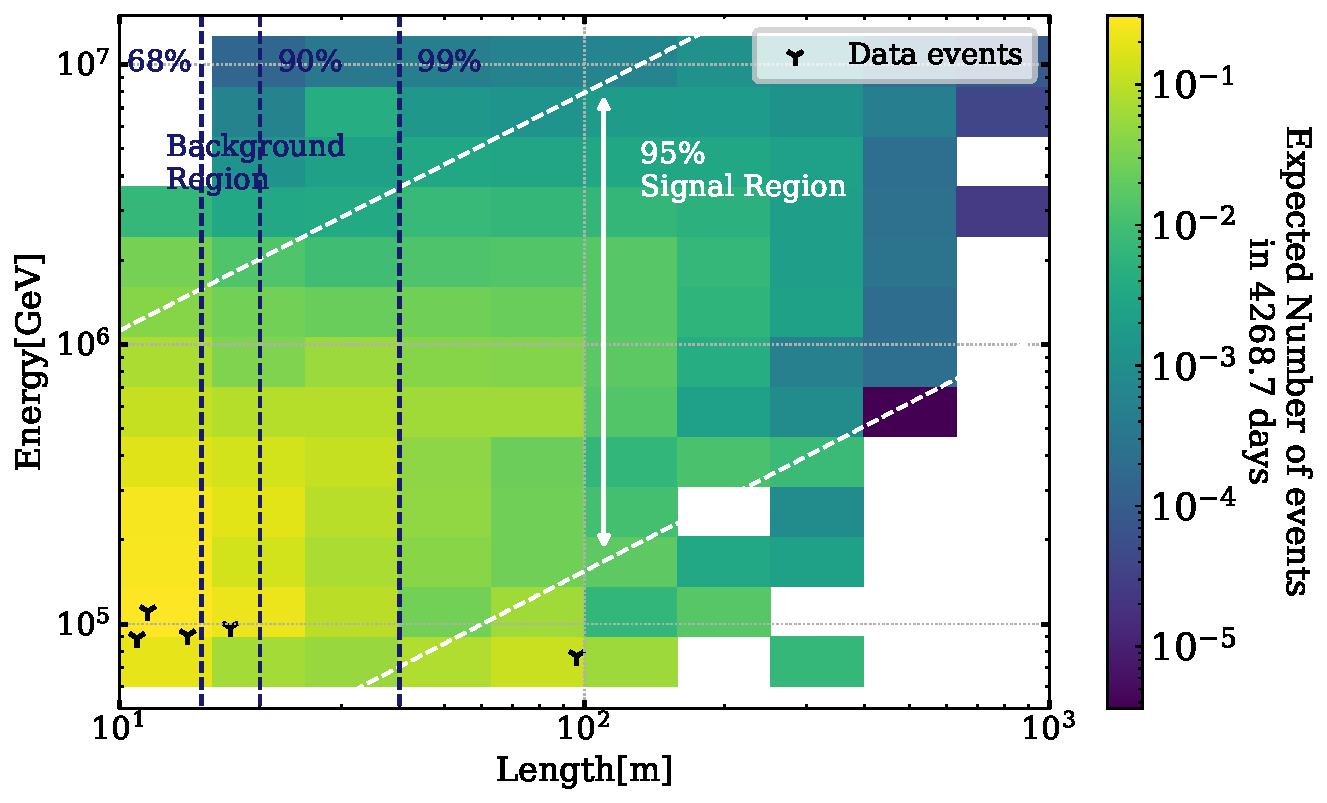
\includegraphics{./figures/results/DataMC_IC86_pass2_SnowStorm_v2_Bfr_DoubleCascadesLvsE_2D_withData.pdf}
    \end{subfigure}
    
    \caption{Two-dimensional distribution of reconstructed energy vs reconstructed double cascade length of the monte carlo events classified as double cascades. Monte carlo sum is produced using all the bestfit parameters from the \reftab{bf_signal} and \reftab{bf_nuisance}. Position of the data events are marked with \wye[rotate=180]. Signal (white) and Background (dark blue) dominated regions are marked with their respective percentiles.}
    \labfig{LvsE_datamc}
\end{figure*}

\begin{marginfigure}
    
    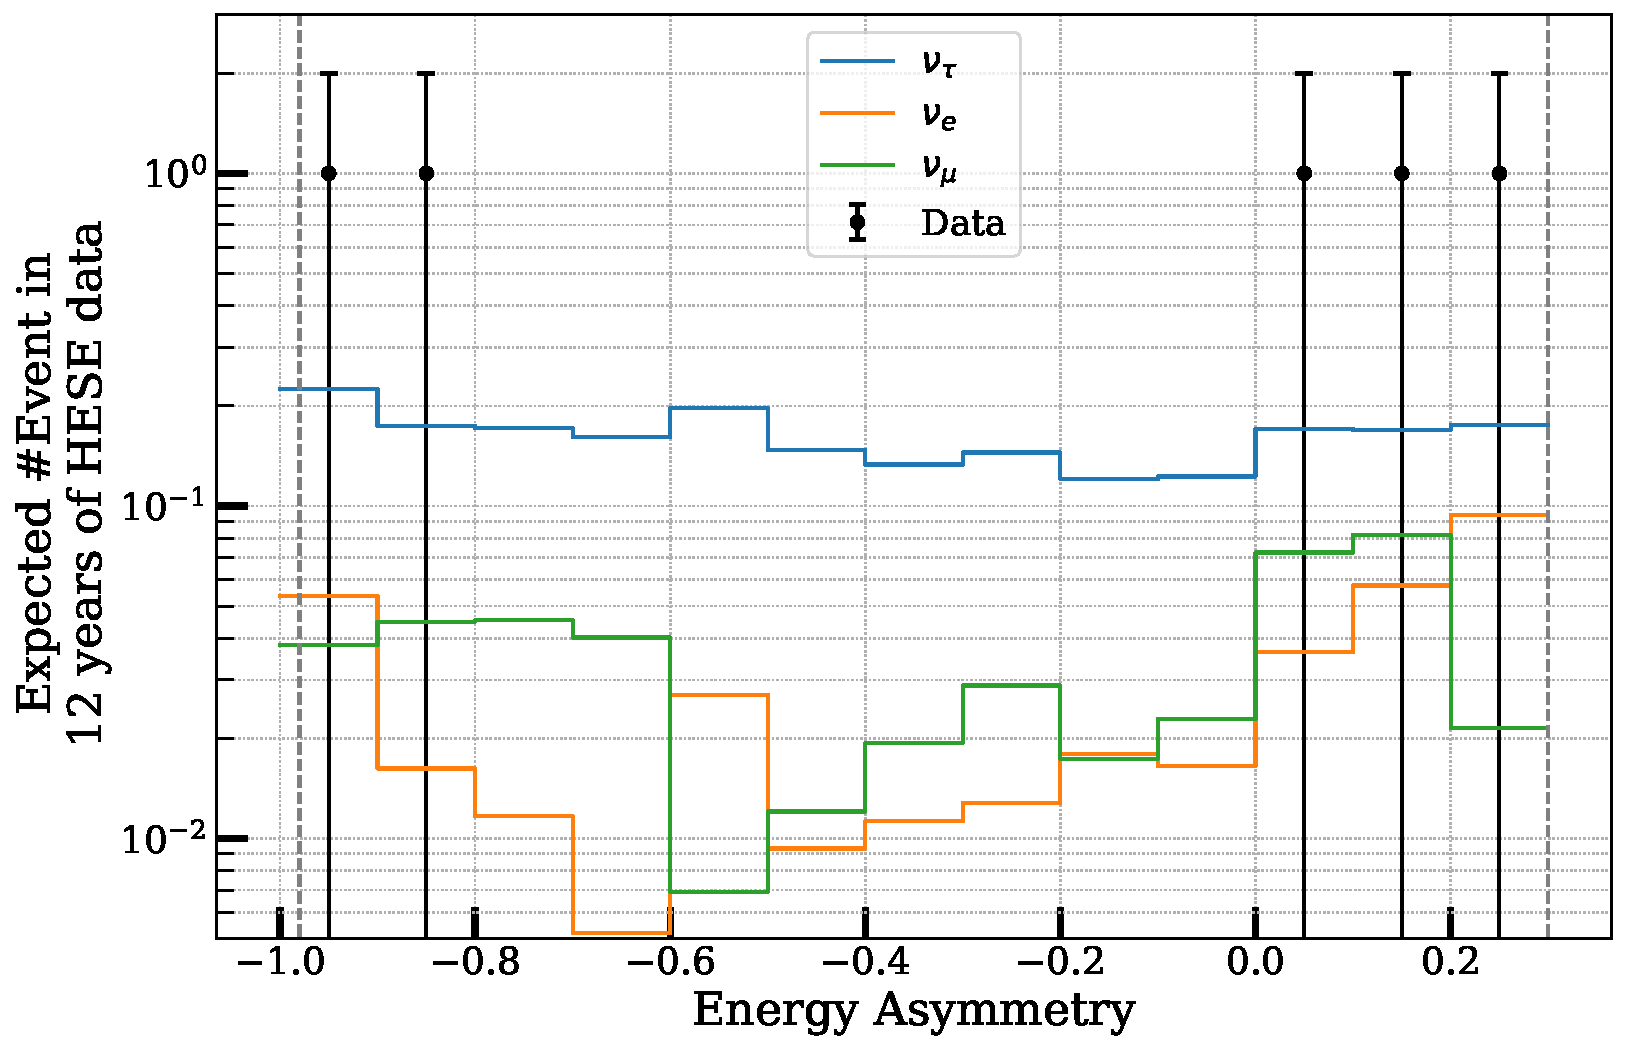
\includegraphics{./figures/results/Energy_ratio.pdf}
    
    \caption{Distribution of reconstructed energy asymmetry, defined as $\mathrm{E}_{\mathrm{A}}=\frac{\mathrm{E}_1-\mathrm{E}_2}{\mathrm{E}_1+\mathrm{E}_2}$, (where $\mathrm{E}_1$ and $\mathrm{E}_2$ are energies of first and second cascades, respectively) at best-fit, along with data events. Distribution is shown for all flavours separately, to emphasis domination of $\nu_{\tau}$ double cascades in the signal region (verticla grey lines).}
    \labfig{Eratio}
\end{marginfigure}

\reffig{Eratio} presents the distribution of the reconstructed energy asymmetry for simulated events in the double-cascade sample, using the best-fit astrophysical and atmospheric spectra. The two vertical lines represent the selection cuts applied to choose the double cascade events, as described in section 4.3. Although two of the 5 events are near the cut edge, they all still fall comfortably within the signal-dominated region of the sample.

\section{Flavour Composition of Diffuse Astrophysical Neutrinos}
\label{sec:flavour_results}
The flavor composition of astrophysical neutrinos is measured using 97 high-energy starting event (HESE) events, which are divided among three morphologies. The profile likelihood scans for the flavor scale factors, specifically $s_{\nu_{e}}$ and $s_{\nu_{\tau}}$, are shown in \reffig{1d_llh}. The results indicate that the tau scale factor ($s_{\nu_{\tau}}$) is only able to reject the possibility of no $\nu_{\tau}$ flux by $1\sigma$ ($-2\Delta \log L=1$), as reflected in the wide contours in the 2D scan shown in \reffig{flavour_comp}. The 1D scans are used to derive $1\sigma$ (68\%) confidence regions, shown in \reftab{bf_signal}. The test statistic $-2\Delta \log L$ compares the global best-fit values of the unconstrained fit to the conditional best-fit values of all remaining model parameters at a fixed scan point. The confidence regions depicted in \reffig{flavour_comp} are calculated using Wilk's theorem \sidecite{Wilks_thm} , as a full Feldman-Cousins construction of the entire flavor composition phase space is computationally demanding (see section \ref{sec:analysis} for details). The agreement of Wilk's theorem is verified by comparing the coverage of the test statistic distribution from Monte Carlo pseudo-experiments to the coverage of a $\chi^2$-distribution. A large fraction of the flavor composition phase space is found to be slightly over-covered, indicating that Wilk's theorem yields a conservative confidence region. Although a part of the 90\% confidence region seems to suffer from slight under-coverage, the $\chi^2$-approximation is deemed sufficient for presenting the measurement result in \reffig{flavour_comp}. 
\begin{figure}
    
    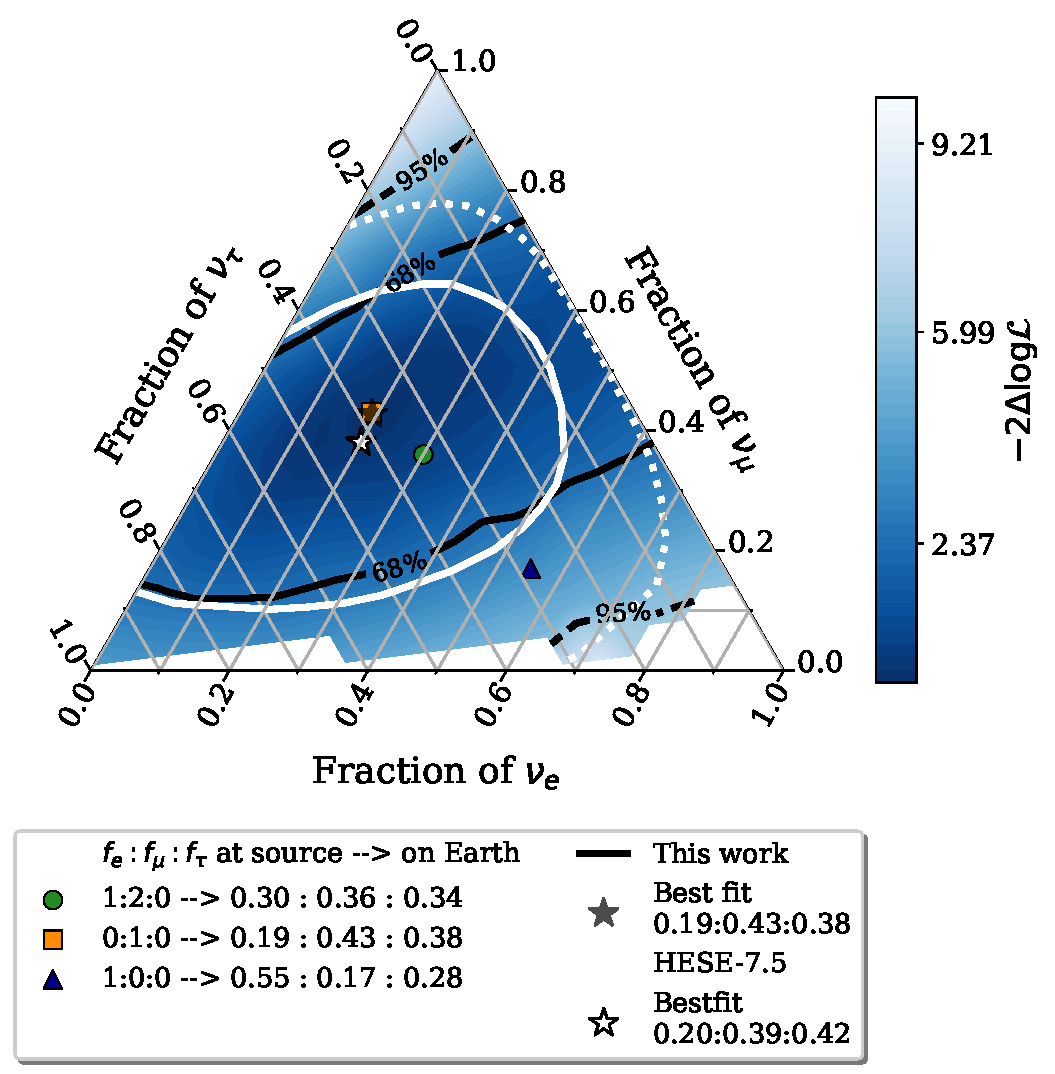
\includegraphics{./figures/results/HESE12_fancy_coverage_say_withhese7.pdf}
    \caption{A 2 dimensional profile likelihood scan of the astrophysical neutrino flavor composition at Earth using 12 years of HESE data, classified in three event morphologies (see text for details). Each point on the triangle corresponds to a flavor composition of $\nu_e : \nu_{\mu} : \nu_{\tau}$ which can be read off the axes along the tick directions specified. The best-fit flavor composition of 0.19 : 0.43 : 0.38 is indicated with a white star. The white solid and dashed lines represent the 68\% and 95\% confidence regions, respectively, obtained from the $\chi^2$-approximation using Wilk's theorem. Three flavor compositions expected at Earth from different source scenarios are also marked (\ref{sec:cosmic_nu}). The best-fit flavor composition of a previous measurement that used 7.5 years of HESE data is indicated in grey star, with the 68\% and 95\% confidence regions represented by the grey solid and dotted lines, respectively \cite{Juliana_paper}.}

    \labfig{flavour_comp}
\end{figure}

\begin{figure*}[h!]
    \begin{subfigure}[h]{0.7\textwidth}
        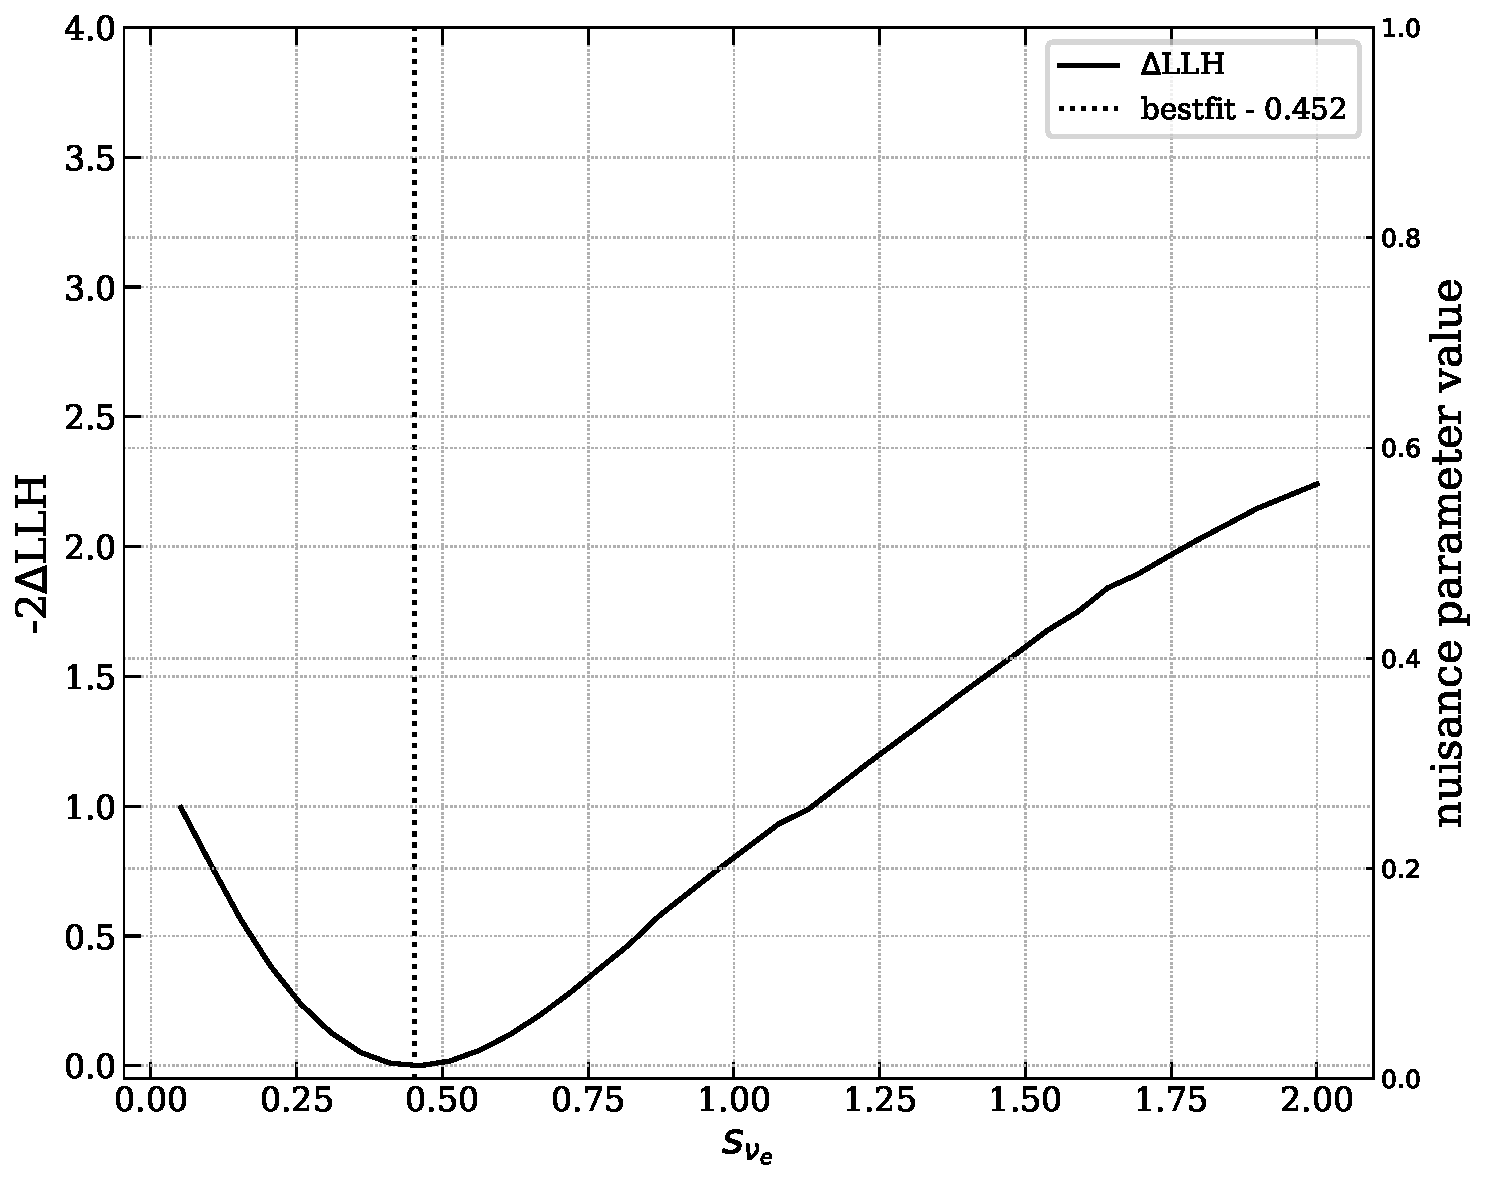
\includegraphics{./figures/results/profile_scan_astro_nue_ratio.pdf}
    \end{subfigure}
    \hfill
    \begin{subfigure}[h]{0.7\textwidth}
        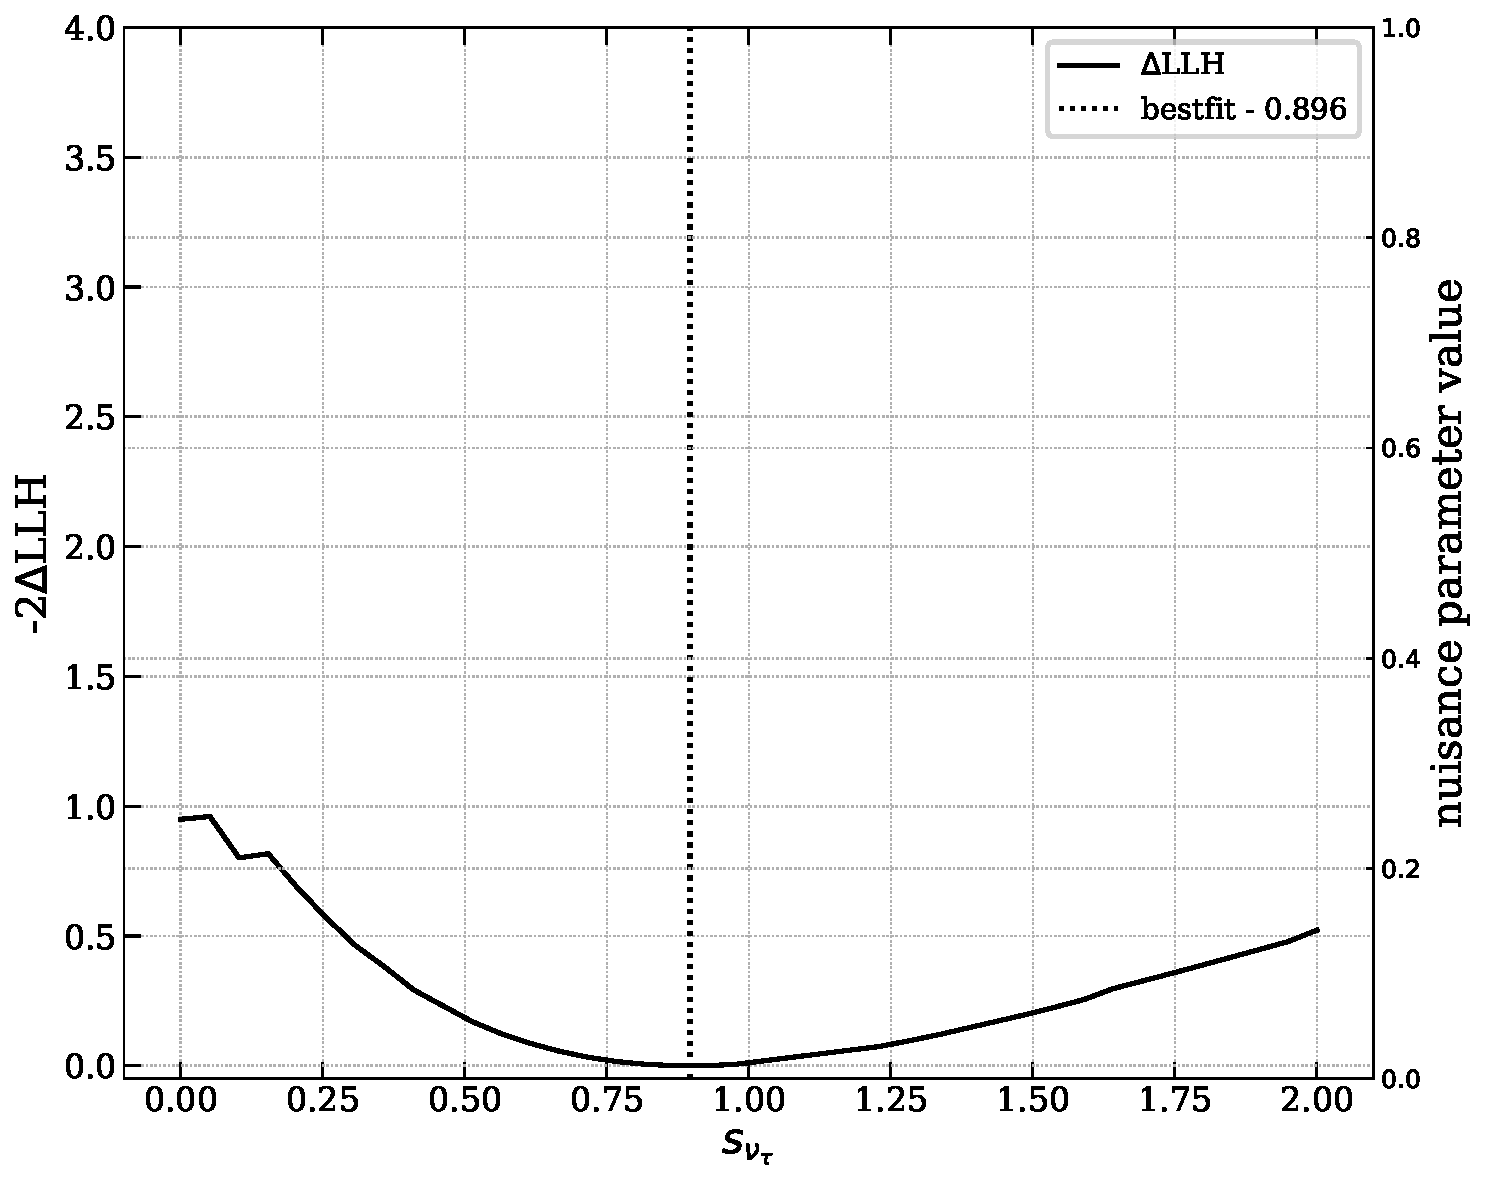
\includegraphics{./figures/results/profile_scan_astro_nutau_ratio.pdf}
    \end{subfigure}
    
    \caption{1 dimensional profile likelihood scan of flavour scale factors $s_{\nu_{e}}$ (left) and $s_{\nu_{\tau}}$ (right). Solid black line corresponds to the profile likelihood, defined by the likelihood ratio $-2\Delta\mathrm{log}\mathcal{L}$ comparing a fixed value to the best-fit value (denoted by dotted line).}
    \labfig{1d_llh}
\end{figure*}

\subsubsection{Why are the limits worse than the previous measurements?}

The best-fit flavor composition $\nu_e:\nu_{\mu}:\nu_{\tau} = 0.19:0.43:0.38$ aligns well with the previous measurement \sidecite{Juliana_paper} of $\nu_e:\nu_{\mu}:\nu_{\tau} = 0.20:0.39:0.42$ (grey lines in \reffig{flavour_comp}). However, with 4 more years of data, which includes more double cascade events, it raises the question of why the limits are not as good. The reason is quite simple, the grey contours are derived using an extended likelihood, based on density estimates by producing a large number ($\sim10^6$ events per particle) of resimulations of 2 classified double cascades to assess the \textbf{tauness} . A dedicated algorithm (\texttt{RODEO}) was developed and used to compute the density estimate for sparse datasets produced from these resimulations in multiple dimensions (see \sidecite{Juliana_thesis} for details). This updated likelihood can be seen as the unbinned, higher-dimensional version of evaluating the contributions of signal-like and background-like events, which was carried out in a two-dimensional binned way (just as done for the analysis presented in this thesis).\marginnote{\begin{kaobox}[title=\textbf{\emph{tauness}}]
    "Tauness" refers to the Bayesian posterior probability that an event is derived from a $\nu_{\tau}$ interaction. This can be approximated by analyzing the fraction of events in close proximity to the reconstructed properties of the data events, which are anticipated to result from $\nu_{\tau}$ interactions. In essence, tauness provides insight into the probability of each double cascade originating from a $\nu_{\tau}$ interaction compared to any other type of interaction.
\end{kaobox}}  Because of this, the limits one should actually compare with the previous measurement should be the one derived using \emph{the non-extended likelihood}, which is the same likelihood and PDF setup used for this iteration of the analysis. \reffig{HESEall68} shows such a comparison. The best-fit flavor composition $\nu_e:\nu_{\mu}:\nu_{\tau} = 0.19:0.43:0.38$ measured using this analysis (black lines) aligns well with the previous measurement of $\nu_e:\nu_{\mu}:\nu_{\tau} = 0.29:0.43:0.28$ (blue lines) using the same likelihood. Although not significantly, the limits derived from this iteration do get better along the $\nu_{\mu}$ fraction. Only 68\% limits are shown, without the likelihood space to keep the plot easy to read.

\begin{figure}[h!]
    \caption{The best-fit flavor composition of 0.19 : 0.43 : 0.38 (black), using 12 years of HESE data (this work) compared with the best-fit flavor composition of a previous measurement that used 7.5 years of HESE data \cite{Juliana_paper}. Comparison is shown by usingth esame likelihood formulation (none extended likelihood without resimulations, see text for details). The solid and dashed lines represent the 68\% and 95\% confidence regions, respectively, obtained from the $\chi^2$-approximation using Wilk's theorem. Three flavor compositions expected at Earth from different source scenarios are also marked (\ref{sec:cosmic_nu}).}
    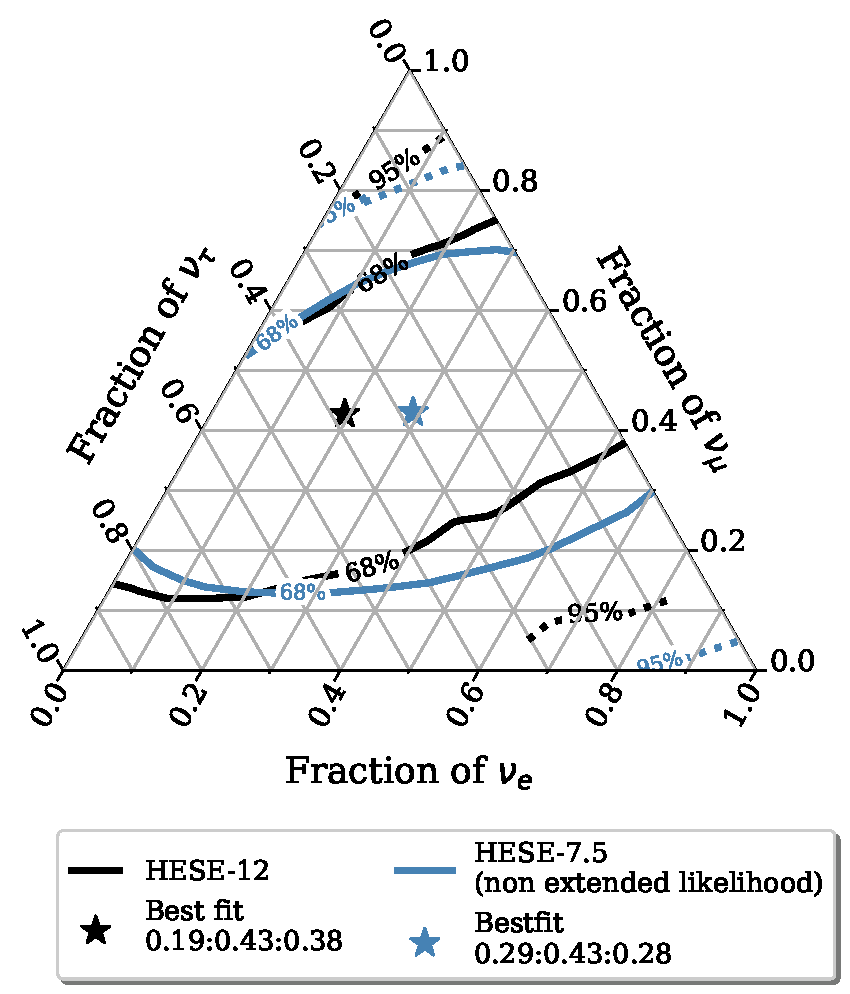
\includegraphics{./figures/results/HESE7and12_nonextendedonly.pdf}


    
    \labfig{HESEall68}
\end{figure}


\subsubsection{Sensitivity at BestFit}
\label{sec:sens_bf}
Please remember the following text:

The setup and all the relevant updates to the sample and selection chain for the analysis presented in this thesis were done using the best-fit values from the previous analysis. The two signal parameters that affect the flavor measurement, especially the $\nu_{\tau}$ fraction and hence the double cascade events, are the index of the primary neutrino energy spectrum $\gamma_{\mathrm{astro}}$ (assuming a single power law) and the normalization. A harder spectrum (low $\gamma_{\mathrm{astro}}$) leads to a higher expected flux, resulting in more expected events, while a softer spectrum (high $\gamma_{\mathrm{astro}}$) leads to a lower flux for samples with a similar effective area. This point was discussed in section \ref{sec:sensitivty} while discussing the sensitivity of the analysis. The analysis setup and sensitivity were shown using a spectrum with an index of 2.87, which is almost identical to the best-fit value for this analysis (2.84) assuming equal partition of the neutrino flavor ($\nu_e : \nu_{\mu} : \nu_{\tau} = 0.33 : 0.33 : 0.33$). Even though the measured flavor ratio is slightly different, the index remains quite close to what the data agrees with, and the estimated sensitivity projected much tighter constraints on 2D flavor measurements, specifically along the $\nu_{\tau}$ axis \todo{cite sensitivity figure here}. To understand the lack of improvement to reduce degeneracy along the $\nu_{e}$/$\nu_{\tau}$ axis, the sensitivity of the flavor measurement was first tested at the best fit.

\begin{marginfigure}
    
    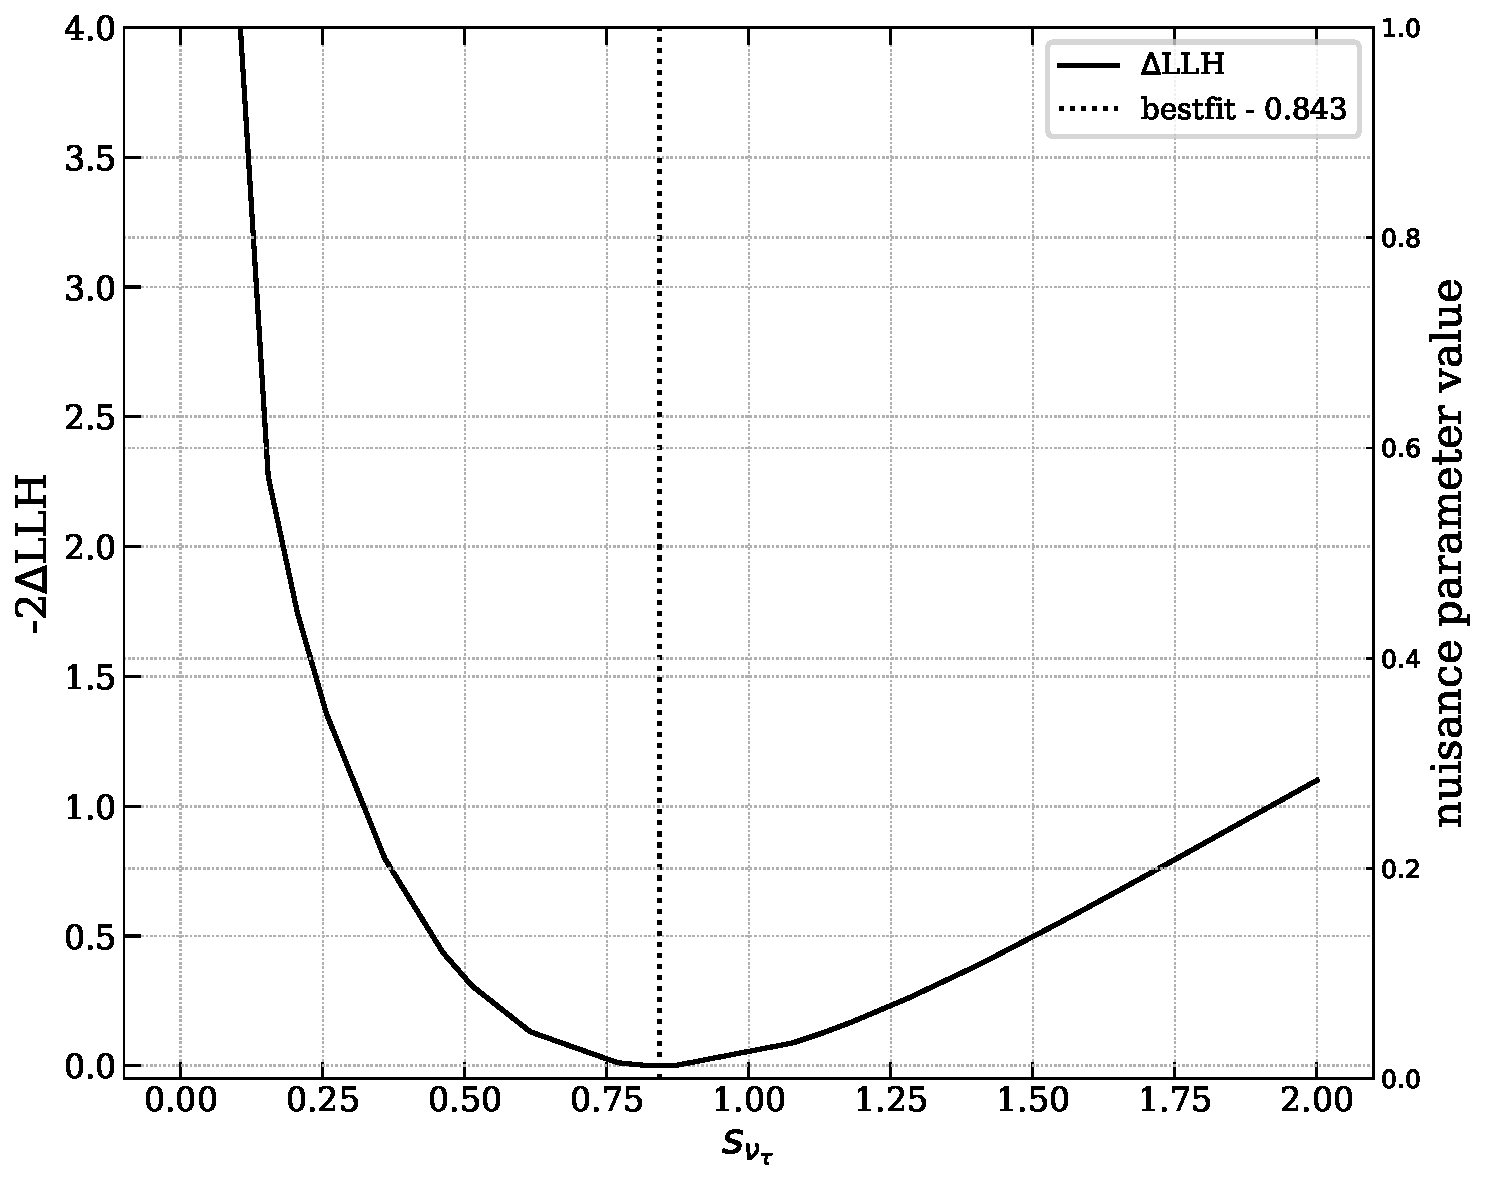
\includegraphics{./figures/results/simulation_profile_scan_astro_nutau_ratio.pdf}
    
    \caption{1 dimensional profile likelihood asimov scan of $\nu_{\tau}$ scale factor, $s_{\nu_{\tau}}$ using \textbf{simulation} injected at bestfit point. Solid black line corresponds to the profile likelihood, defined by the likelihood ratio $-2\Delta\mathrm{log}\mathcal{L}$ comparing a fixed value to the best-fit value (denoted by dotted line).}
    \labfig{profile_llh_nutau_sim}

\end{marginfigure}

The sensitivity of the bestfit analysis is demonstrated in \reffig{PEs}. It is determined by using an asimov dataset \sidecite{asimov} created with the best-fit values of all signal and nuisance parameters from \reftab{bf_signal} and \reftab{bf_nuisance}. For the sake of simplicity in comparison, a Poisson likelihood was utilized, as SAY likelihood tends to yield more conservative limits (refer to the appendix for some comparisons). The objective here is to examine the most ideal scenario. Moreover, constructing pseudotrials where data is drawn from SAY likelihood is not straightforward, therefore, to maintain consistency in comparisons, all fits depicted in \reffig{PEs} are computed using Poisson Likelihood. Consequently, the 68\% data limits displayed on the same plot (black line) are narrower compared to those shown in \reffig{flavour_comp}. Additionally, there is a slight shift in the bestfit point. The key point here is that, given these signal parameters, the analysis is sensitive not only to measure a non-zero $\nu_{\tau}$ fraction, but also to reject it with better significance (approximately $3\sigma$ as shown in \reffig{profile_llh_nutau_sim} - the 1D profile likelihood scan of $s_{\nu_{\tau}}$ for the asimov dataset used to derive the 2D limits shown in \reffig{PEs}). The sensitivity results give rise to three questions:

\textbf{Are data limits reliable?}\\
The contours shown in \reffig{flavour_comp} are based on the assumption that Wilk's theorem holds. This theorem states that the $-2\Delta\mathrm{log}\mathcal{L}$ approximately follows a $\chi^2$-distribution with $k = \text{dof}(\hat{\theta}, \hat{\xi}) - \text{dof}(\theta_t, \xi_t)$, where $\text{dof}(\theta, \xi)$ represents the number of free parameters in the fit. In the case of the flavour fit, there are 2 free parameters - $s_{\nu_{e}}$ and $s_{\nu_{\tau}}$. It is important to note that Wilk's theorem is only valid if the sample size is large and the model parameters are not bounded. However, the HESE sample is relatively small with only a few events passing all selection cuts. Additionally, the available Monte Carlo statistics are not large enough to provide sufficient statistics in every bin of the analysis histograms. Furthermore, the parameters are bounded as the flavour fractions cannot be negative. Therefore, it is essential to verify the validity of Wilk's theorem given these conditions.
     
\textbf{Is deriving sensitivity using an asimov dataset a good choice?}\\
The Asimov dataset is a convenient alternative to generating a large number of pseudo trials for testing a specific realization. Computing the test statistic distribution of both conditional and global best-fit values for each point in the triangle is quite expensive. It should not be assumed that the test statistic value that maximizes the likelihood of the Asimov dataset is always equal to the median of the test statistics derived from the full distribution of various pseudo experiments. Therefore, the next step is to calculate sensitivity using Monte Carlo pseudo experiments.

\textbf{Is the 2 dimesnional monte carlo PDF ideal for the fit to differentiate between signal and background?}\\

Forward-folding fits, as described in section \ref{sec:analysis}, heavily relies on the expected values for each bin of the analysis histograms. It is crucial to choose reliable variables so that the likelihood space looks different for signal and background. For this reason, the analysis variables for double cascade bins are different from those for cascades and tracks. This is because the zenith distribution of astrophysical $\nu_{\tau}$ flux shows no significant variation between signal and background. The PDF used in this case was selected due to the correlation of the Tau decay length ($\mathrm{L}_{\mathrm{dc}}$) with the energy of the second cascade ($\mathrm{E}_{2}$) for double cascades resulting from $\nu_{\tau}$-cc interactions, contributing to the population of signal events along this diagonal \todo{reference PDFs from the analysis chapter}. The 2D Monte Carlo PDF at best fit, shown in \reffig{LvsE_datamc}, contains Monte Carlo events populating the bins along the diagonal. However, the data events are in regions where the background population is expected with nearly equal probability. While drawing data using poisson distribution, fluctuations around the best-fit are considered which in principle should give all possible realisations of the data events ending up in bins with high expectations \sidenote{This was also the motivation beg=hind the resimulations that were performed for the previous iteration of the analysis to measure the flavour composition}. Since data events are observed in bins with not so high expectations as well, it may happen that most pseudo trial histograms would end up not replicating data event distributions. Therefore, in addition to the pseudotrials described earlier, the histograms produced for each trial were checked to see how often the events ended up in a region mostly occupied by background-like events. 

\begin{marginfigure}
    
    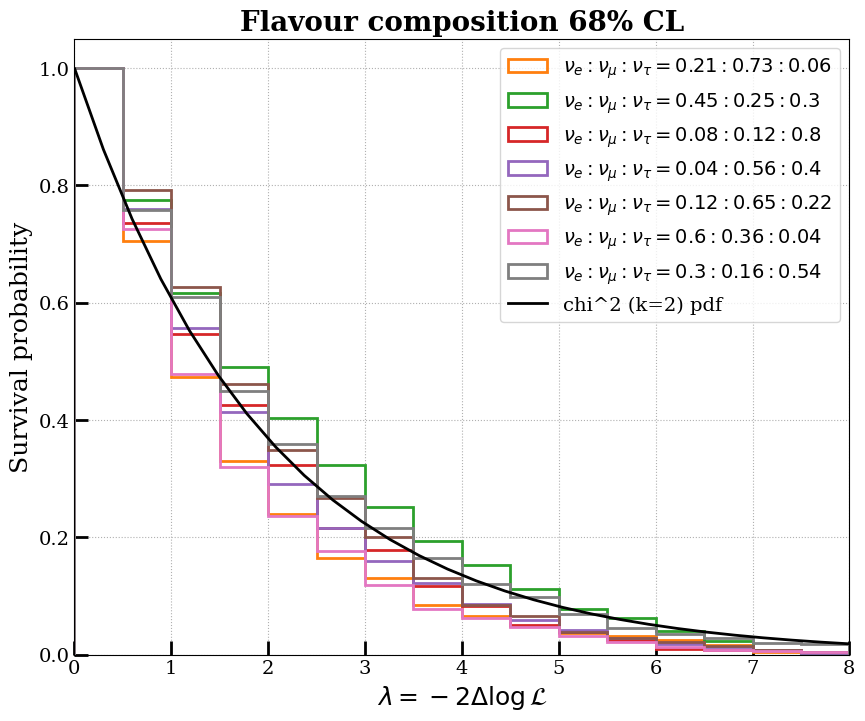
\includegraphics{./figures/results/wilk's test.png}
    
    \caption{Test statistic distribution of the pseudo datasets. All datasets are injected at set of points on 68\% contour (solid white line) of \reffig{flavour_comp} (also shown in legend). a $\chi^2$-distribution with 2 degrees of freedom is also shown (black line) for refernece.}
    \labfig{wilks_68}

\end{marginfigure}

Both of these tests were conducted and their detailed descriptions are provided in Appendix A. The validity of Wilk's theorem was tested for a few points on the 68\% and 95\% contours. This was achieved by generating pseudo datasets (500 trials per dataset), each injected with a specific flavor composition (a point on the contour), while keeping the rest of the fit parameters at their best-fit values. Each trial was fitted twice: once by keeping the parameters fixed at the injection point and once with them free. A likelihood ratio test was performed for each trial by taking the ratio of free to fixed likelihood values. The results are represented in a TS distribution shown in Figure A (for points on the 68\% line). For comparison, a $\chi^2$-distribution with 2 degrees of freedom is also shown (black line). The TS distribution of some points shows a minor shift from the $\chi^2$ (k=2) case, but nevertheless, shows no significant violation of Wilk's theorem.


\begin{figure}[h]
    
    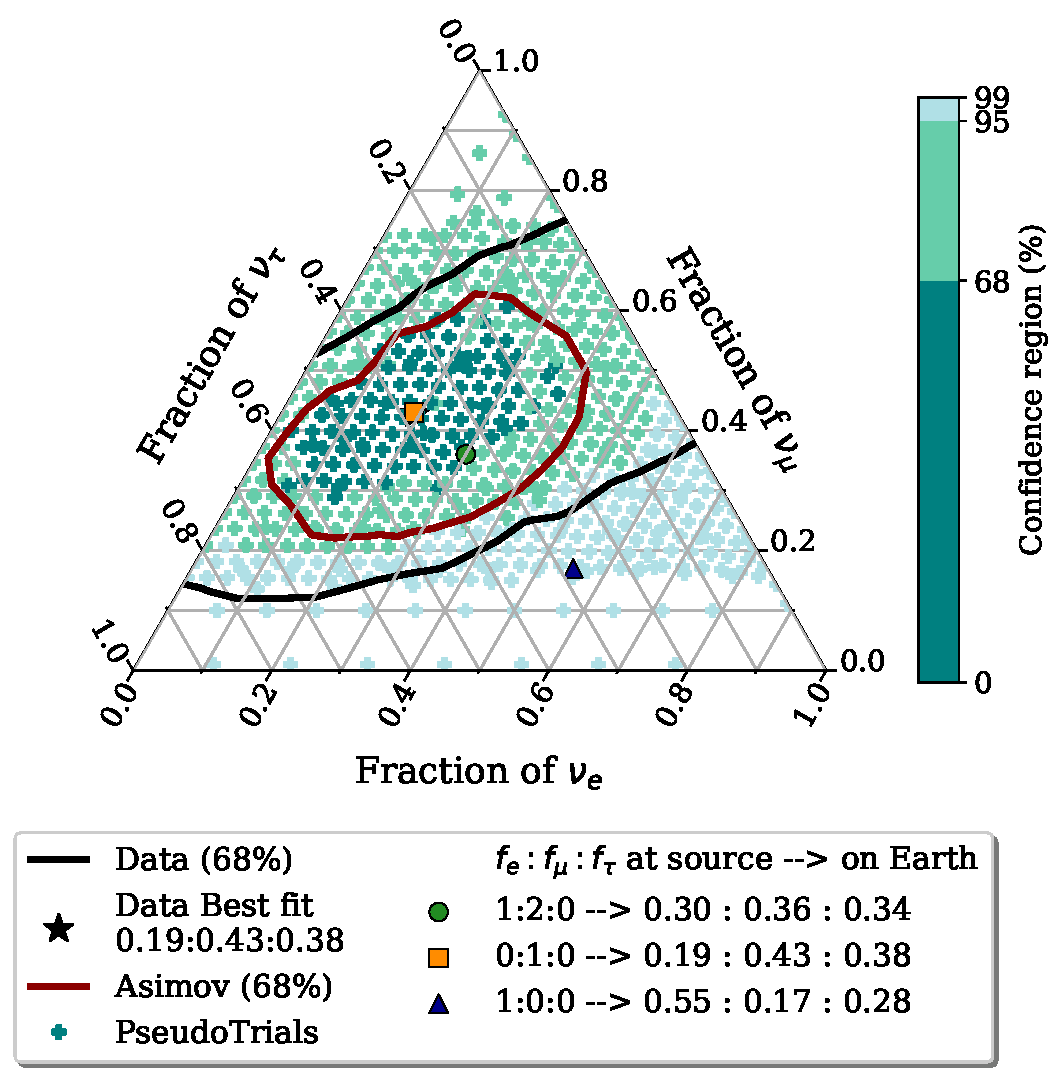
\includegraphics{./figures/results/PE_data_asimov_68.pdf}


    \caption{Comparison of Measured flavoured ratio (black line) with asimov sensitivity(maroon line) and pseudo trials (marked with '+'). Each + represents a pseudo dataset, drawn from flavour composition of that very point. Colorbar shows confidence intervals of each of these points, to reject the bestfit flavour composition of $\nu_e:\nu_{\mu}:\nu_{\tau} = 0.19:0.43:0.38$. All other parameters of the fit are injected at their bestfit values.}
    \labfig{PEs}
\end{figure}

The second test was conducted in a similar way, but this time the fixed point for all trials was kept at the data best-fit point. In Figure B, each point denoted with a marker "+" represents the points for which pseudo datasets were generated. Each dataset was generated by injecting the point denoted with "+" and fitted twice: once by keeping $s_{\nu_{e}}$ and $s_{\nu_{\tau}}$ fixed at the data best-fit values (from \reftab{bf_signal}) and once with them free. This was done to test if the true flavor fraction is what the data fit returns and with what confidence the injected point can be rejected. The result is shown in Figure B. The color scheme shows the confidence level each point has to reject the null hypothesis (data best-fit in this case). As can be seen, the pseudo-trial distribution matches quite well with the Asimov sensitivity. In fact, it predicts even tighter constraints compared to the Asimov case, indicating that neither data limits nor Asimov limits are unreliable.

Lastly, the aforementioned third point was checked. Ideally, one would generate pseudo trials until all the Poisson-distributed events fall within the same region of the PDF as shown in \reffig{LvsE_datamc}. However, this approach was found to be computationally expensive. For instance, each dataset displayed (around 400) in \reffig{PEs} was produced from 500 trials, with each trial fitted twice. On average, each fit took approximately one hour to complete. Therefore, before proceeding, the proportion of PDFs that did not meet the cut criteria was estimated to determine whether using computational resources for further trials was justified. Several tested datasets from different regions of the triangle revealed that, for most datasets, only about 20\% of the 500 trials resulted in final histograms with events concentrated in the lower energy bins. There was no feasible way to generate a sufficient number of trials to reduce statistical errors and set definitive limits. As a workaround, only the small proportion of trials that met the necessary criteria were used to generate the TS distributions, allowing an update of the sensitivity shown in \reffig{PEs}. This updated result is presented in \reffig{PEs_bkg}. As evident from the vanished points, not only were most of the trials excluded, but the confidence intervals also became significantly larger—especially along the $\nu_{\tau}$ axis—aligning more closely with the data limits. This concludes why both asimov sensitivity and pseudo trials in \reffig{PEs} showed such tight constraints. In an ideal case, one can perform resimulations of the 5 double cascade events as it was done for the previous iteration, but this would in turn increase computational resources and was beyond the timeline of work presented in this thesis, hence it was not performed.


\begin{figure}[h]
    
    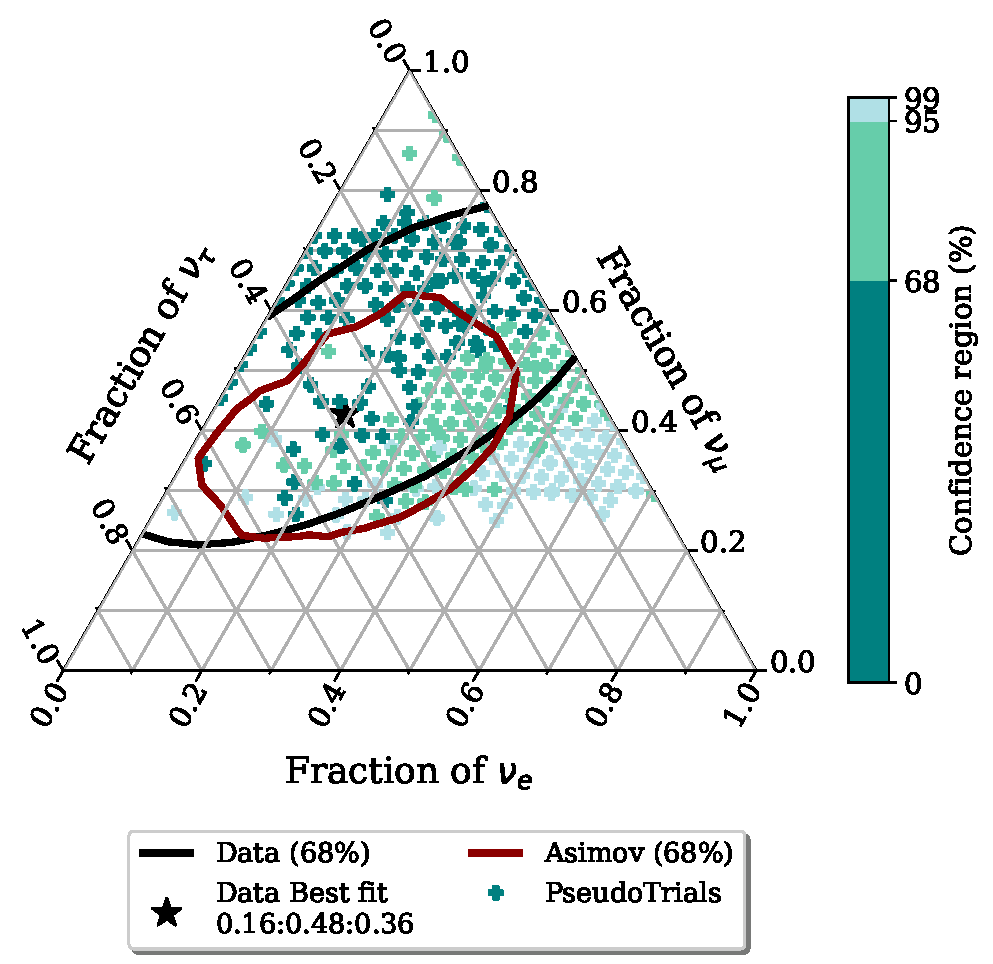
\includegraphics{./figures/results/PE_data_asimov_68_BkgOnly.pdf}


    \caption{Comparison of Measured flavoured ratio (black line) with asimov sensitivity(maroon line) and pseudo trials (marked with '+'). Each + represents a pseudo dataset, drawn from flavour composition of that very point. Colorbar shows confidence intervals of each of these points, to reject the bestfit flavour composition of $\nu_e:\nu_{\mu}:\nu_{\tau} = 0.19:0.43:0.38$. Only trials with final histogram in three lower energy bins are kept in TS distribution. All other parameters of the fit are injected at their bestfit values.}
    \labfig{PEs_bkg}
\end{figure}

\section{Discussion}
\label{sec:results_discussion}

The analysis setup and particle identification methods developed and refined throughout this thesis demonstrate that IceCube is sensitive enough to measure the flavor ratios of the astrophysical neutrino spectrum and set tight constraints. However, more robust techniques, particularly for reconstructing double-cascade events, are needed to produce more reliable Monte Carlo PDFs for these fits. Regarding the measured flavor ratio, as shown in \reffig{Flavour_comp}, although the best fit suggests neutrinos are produced by the muon-damped scenario at high-energy sources, no other source scenarios can be excluded with high significance. The neutron beam scenario ($\nu_e:\nu_{\mu}:\nu_{\tau} = 1:0:0$ at the source, evolving to 0.55:0.17:0.28 on Earth) is disfavored by approximately $1\sigma$ but remains consistent at $2\sigma$.

A specific measurement of the neutrino energy spectrum was not part of the analysis presented here, as the focus was primarily on flavor measurement, with efforts directed toward improving particle identification. Nonetheless, the HESE sample could also be used to measure, and potentially search for, spectral features. Recent independent studies have discovered a spectral break in the neutrino spectrum at around 30 TeV, softening the spectrum at higher energies, which is within the range of this analysis \sidecite{globalfit_icrc,MESE_icrc}. This finding offers insight into why previous measurements targeting different energy ranges produced significantly different spectral indices for a single power-law spectrum \sidecite{HESE7_sample,diffusenumu,cscd_6yr}. Since the HESE sample focuses on high-energy events, where no such spectral features have been observed, and has much lower statistical power than those other samples, no spectral feature searches were attempted during this thesis work.

A less model-dependent approach to describing the astrophysical neutrino flux is the differential unfolding of the energy spectrum. This method divides the flux into energy bins, where each bin is fit independently with a constant $\sim\mathrm{E}^{-2}$ spectrum, rather than assuming a continuous power-law across the entire energy range. Ideally, this unfolding would be performed separately for each neutrino flavor to avoid assuming a uniform spectral shape for all flavors. Measuring the flavor composition as a function of energy would also be valuable, as neutrino production processes are energy-dependent. However, due to the limited statistical power of the current dataset, meaningful results could not yet be obtained.

Finally, improvements in reconstruction methods and more data are necessary for future experiments to shed more light on flavor measurements. Double-cascade reconstruction currently has an upper energy limit, as higher-energy events are only partially contained within the detector due to their geometry. In addition, improved detection hardware could provide better information on photon charge and direction, enhancing the overall reconstruction process. These points, along with the potential for a proposed new generation of neutrino detectors, will be discussed in detail in the next chapter. 


% In particular, various issues encoutered, ice model effects, using high quantum efficiency DOMs, etc need to be studied in more detail. The reconstruction and classification algorithms were desgined and developed while neither detector nor detecting medium was well understood. With more than 10 years of data, the statistical uncertainties are reducing significantly, revealing interesting physics (for both neutrinos and detector). Using all of this new information, the selection can be made more robust against changes like use of DOMs, icemodels etc. 
